%&encoding=UTF-8 Unicode
\documentclass[12pt,twoside,openany]{fithesis}
\usepackage[resetfonts]{cmap}


% Nastavení fontů.
\usepackage{palatino}

\pdfpkresolution=1200
\usepackage{cmap}

\usepackage[lmargin=35mm,
	        rmargin=25mm,	
            tmargin=25mm,
            bmargin=30mm,
            includeheadfoot,
            heightrounded,
           ]{geometry}

\usepackage[czech]{babel}
\AtBeginDocument{\shorthandoff{-"}} % Deaktivuje znaky spojovník (-) a uvozovky 
                              % (") aktivované novou podporou češtiny v balíčku 
                              % "babel", což zabrání problémům se zadáváním 
                              % těchto znaků v parametrech některých maker.
\usepackage[utf8x]{inputenc}
\usepackage[T1]{fontenc}
\usepackage[isu,small,bf,up]{caption}
\usepackage{pdfpages}


\usepackage{tocloft}

%fasrhdfhdhatdh \usepackage[labelformat=Obrázek]{caption}

\pdfpkresolution1200
\usepackage[protrusion,expansion,step=1]{microtype}
\usepackage[unicode=true,
            colorlinks=true,
            plainpages=false,
            pdfpagelabels=true,
            %pdfborder={0 0 0},
            %backref=page,
            pdfpagemode=UseNone,
            pdfstartview={XYZ null null 1},
            pdfpagelayout=OneColumn,
            pdfdisplaydoctitle=true,
            bookmarks=true,
            bookmarksopen=true,
            bookmarksopenlevel=5,
            bookmarksnumbered=true
           ]{hyperref}

\makeatletter
    \let\origsection\section%
    \def\section{%
        \@ifstar%
            {\starsection}%
            {\origsection}}%
    \def\starsection#1{%
        \origsection*{%
            \phantomsection%
            \addcontentsline{toc}{section}{#1}%
            #1}}%
    \let\origsubsection\subsection%
    \def\subsection{%
        \@ifstar%
            {\starsubsection}%
            {\origsubsection}}%
    \def\starsubsection#1{%
        \origsubsection*{%
            \phantomsection%
            \addcontentsline{toc}{subsection}{#1}%
            #1}}%
    \let\origsubsubsection\subsubsection%
    \def\subsubsection{%
        \@ifstar%
            {\starsubsubsection}%
            {\origsubsubsection}}%
    \def\starsubsubsection#1{%
        \origsubsubsection*{%
            \phantomsection%
            \addcontentsline{toc}{subsubsection}{#1}%
            #1}}
\makeatother
\makeatletter
    \def\cleardoublepage{\clearpage\if@twoside \ifodd\c@page\else
        \thispagestyle{empty}
        \hbox{}\newpage\if@twocolumn\hbox{}\newpage\fi\fi\fi}
\makeatother
\mathcode`\,="013B
\def\,{\kern 0.25em}
\newcommand{\tecky}{\kern 0.16667em\dots}
\newcommand{\cssplit}[1]{\discretionary{#1}{#1}{#1}\kern 0pt}
\newcommand{\spj}{\cssplit{-}}
\newcommand{\sls}{\cssplit{/}}
\newcommand{\bsls}{\char`\\}
\let\origurl\url
\def\url#1{\texttt{<\origurl{#1}>}}
\def\email#1{\texttt{<\href{mailto:#1}{#1}>}}
\def\odkaz#1#2{#1 (\url{#2})}
\def\skrytyodkaz#1#2{\href{#2}{#1}}

\widowpenalty10000
\clubpenalty10000
\newcommand{\vhodnyzlom}{\penalty-5000}
\newcommand{\nevhodnyzlom}{\penalty5000}

\setcounter{secnumdepth}{2} %2
\setcounter{tocdepth}{4} %2

\makeatletter
\renewcommand\@makefntext[1]%
    {{\textsuperscript{\@thefnmark}\,}#1}
\makeatother


%%% Informace o práci:
\thesistitle{Affiliate Marketing} % Makro umožní vložit název práce, u dvouřádkových
                   % či víceřádkových názvů se standardně oddělí  jednotlivé
                   % části příkazem \\ s volitelným parametrem meziřádkového 
                   % prokladu.
\thesissubtitle{Bakalářská práce} % Makro umožní vložit název typu práce, např.
                                  % bakalářská práce, diplomová práce atd.
\thesisstudent{Pavel Smolka} % Makro umožní pomocí svého jediného parametru
                             % vložit jméno studenta.
\thesiswoman{false} % Makro umožní vložit pohlaví studenta. Možné hodnoty jsou 
                    % true a false.
\thesisfaculty{eco} % Makro umožní stanovit pod jakou fakultou byla práce 
                   % napsána. Podle toho se také vloží patřičné logo a název 
                   % fakulty na titulní stránku. Jsou podporovány fakulty MU fi, 
                   % sci, law, eco, fss, med, ped a phil. Pokud práce není psaná 
                   % pod žádnou z výše uvedených fakult MU, pak je nutné zadat 
                   % i název univerzity \thesisuniversity{}, jméno souboru loga 
                   % fakulty (bez přípony) \thesislogo{} a též do makra 
                   % \thesisyear{} sídlo dané univerzity (pro MU toto není 
                   % třeba).

\thesisuniversity{Studijní obor: Podniková ekonomika a management}
\thesisyear{2013} % Makro umožní vložit rok vypracování práce.
\thesisadvisor{Ing. Klára Kašparová, Ph.D.} % Makro umožní vložit jméno vedoucího práce.
\thesislang{cs} % Makro umožní stanovit jazyk, ve kterém je práce napsaná
                % (v současné době jsou podporovany variany cs, sk, en).
% Makro pro definici klíčových slov práce.
\def\klicovaslova{\hspace{5mm}
      affiliate marketing, 
      webový marketing, 
      e-shop,
      inovace softwarového produktu,
      e-magazín,
      webový magazín}
\makeatletter
\hypersetup{%
    pdfauthor={\@thesisstudent},
    pdftitle={\@thesistitle},
    pdfsubject={\@thesissubtitle},
    pdfkeywords={\klicovaslova}
}
\makeatother



\begin{document} % Začátek dokumentu.

\FrontMatter % Pro první strany dokumentu obsahující prohlášení, abstrakt 
             % a klíčová slova se nastaví římské číslování.
\ThesisTitlePage % Vysadí titulní stranu práce. Využije předem zadaných údajů 
                 % názvu práce, jména studenta a roku vypracování
\clearpage          




     \begin{figure}[h!]	
\begin{tabular}{l l }\vspace{1mm}
Jméno a příjmení autora:~~~~~	& Pavel Smolka	\\ \vspace{1mm}
Název bakalářské práce:	&	Affiliate Marketing\\ \vspace{1mm}
Název práce v angličtině:	&	Affiliate Marketing\\ \vspace{1mm}
Katedra:	&   Katedra podnikového hospodářství	\\ \vspace{1mm}
Vedoucí bakalářské práce:	&	Ing. Klára Kašparová, Ph.D.	\\ \vspace{1mm}
Rok obhajoby:	&	2014 \\
\end{tabular}
\end{figure}

\vspace{10mm}

\fontsize{18} {26}\textbf{Anotace}
\vspace{3mm} 
\\Bakalářská práce se zabývá problematikou affiliate marketingu z
pohledu velké vydavatelské společnosti. V teoretické části je
popsán princip fungování affiliate marketingu. Dále jsou
vybrány relevantní kapitoly z teorie nákupního rozhodování a
vývoje produktu. V praktické části je analyzován způsob
provádění affiliate marketingu ve vydavatelské společnosti
Future a srovnání s konkurenčními službami. Následuje analýza
výsledků provedeného marketingového výzkumu, na jejichž základě
jsou formulována doporučení týkající se inovace softwarového
produktu.
                                                            
\vspace{5mm}
\fontsize{18} {26}\textbf{Annotation}
\vspace{3mm}
\\The thesis comprehends the topic of affiliate marketing, from
the perspective of a publishing company. The principles of
affiliate marketing are described, along with relevant topics
on purchase decision and product development. According to the
theoretical background, we analyse the current state of
affiliate marketing performance in Future, a publishing
company. Also, a comparison to several competitors is carried
out. Based on a marketing research, the set of recommendations
presents various ways to innovate a software product of the
publisher.

\vspace{15mm}

\fontsize{18} {26}\textbf{Klíčová slova}
\vspace{3mm}
      \\affiliate marketing, 
      webový marketing, 
      e-shop,
      inovace softwarového produktu,
      e-magazín,
      webový magazín
       
\vspace{5mm}
    
\fontsize{18} {26}\textbf{Keywords}
\vspace{3mm}
      \\affiliate marketing, 
      web marketing, 
      e-shop,
      software product innovation,
      online magazine,
      web magazine


\begin{ThesisDeclaration} % Prostředí vysadí stránku s prohlášením o samostatném 
                          % vypracování diplomové práce. Text tohoto prohlášení 
                          % může uživatel předefinovat pomocí makra 
                          % \DeclarationText.

\vspace{20mm}

Prohlašuji, že jsem bakalářskou práci nazvanou Affiliate marketing 
vypracoval samostatně 
pod vedením Ing. Kláry Kašparové, Ph.D. a uvedl v ní všechny použité 
literární a jiné odborné 
zdroje v souladu s právními předpisy, vnitřními předpisy Masarykovy 
univerzity a vnitřními akty 
řízení Masarykovy univerzity a Ekonomicko-správní fakulty MU.

\vspace{20mm}

V Bath, dne 15. května 2014. \hspace{40mm}\hrulefill 

\hspace{105mm} Podpis autora

%\AdvisorName % Vysází údaje o vedoucím práce.
\end{ThesisDeclaration}

\DeclareRobustCommand{\gobblefive}[5]{}
\newcommand*{\SkipTocEntry}{\addtocontents{toc}{\gobblefive}}

\SkipTocEntry\begin{ThesisThanks} % Toto prostředí umožní vysadit poděkování.

\vspace{20mm}

Rád bych na tomto místě poděkoval své vedoucí, paní Kláře Kašparové. 
Nejen za její rady a připomínky k mé bakalářské práci, ale i za 
zaujetí pro marketing, které na mě do značné míry přenesla. Stejně tak 
děkuji všem, kteří mi při studiu pomáhali pronikat do tajů matematiky a 
statistiky, nutných nástrojů při jakékoli analýze dat. 

Jsem vděčný kolegům ze společnosti Future, díky jejichž důvěře
jsem měl v uplynulém roce rozhodovat o nové podobě platformy affiliate
marketingu v této vydavatelské společnosti. Zároveň bych 
chtěl také poděkovat všem svým blízkým za trpělivost, se kterou snášeli, 
když jsem se věnoval studiu a závěrečné práci na úkor času, který 
bych mohl trávit s nimi.

\end{ThesisThanks}
\normalsize




%\MainMatter % Nastaví kromě arabského číslování stránek také implicitní styl 
            % stránky pro sazbu následujících kapitol. V tomto stylu se do 
            % hlavičky stránky vkládá název aktuální kapitoly a od ostatního 
            % textu se záhlaví oddělí horizontální čarou.

%\phantomsection
%\addcontentsline{toc}{chapter}{\textbf{\contentsname}}
%\markright{\contentsname}


\tableofcontents % Vysází obsah.

\MainMatter

% -------------------------------------------------------------
% Chapter Úvod 
% ------------------------------------------------------------- MainMatter
%\chapter*{Úvod}
%\phantomsection
%\addcontentsline{toc}{chapter}{Úvod}
%\markright{\contentsname}

\cleardoublepage
\chapter*{Úvod}
\phantomsection
\addcontentsline{toc}{chapter}{Úvod}
\markboth{Úvod}{Úvod}

Statisíce, miliony, miliardy. V~takových číslech se v~dnešní době 
pohybují počty lidí majících přístup k~internetu. Internet se 
z~původní komunikační sítě vyvinul v~platformu, v~rámci které se 
vzrůstajícím počtem uživatelů roste i množství firem, které v~tomto 
prostředí realizují většinu svého zisku. Jedním z~typických příkladů 
jsou internetové obchody, díky nimž je možno si dnes zakoupit prakticky 
cokoliv online. Jiným druhem společnosti, která spoléhá na internet jako 
médium pro snadné šíření informací, je vydavatelská společnost 
publikující nejrůznější magazíny. Od počátku 21. století je 
celosvětovým trendem pokles popularity tištěných médií -- novin i 
časopisů. To ale nemusí znamenat konec pro jejich vydavatele, pokud se 
dokáží adaptovat a digitalizovat svou nabídku. \cite{decline-of-print}

Málo tištěných novinových či časopisových titulů se mohlo chlubit 
tím, že byly schopny pokrýt veškeré náklady pouze z~tržeb inkasovaných 
prodejem výtisků. Esenciální součástí drtivé většiny z~nich se tak 
staly reklamní a inzerční rubriky. S~nástupem elektronických magaznínů, 
zejména těch, které jsou publikovány přímo na webových stránkách, se 
tento trend ještě zvýšil. Většina čtenárů není zvyklá za obsah na 
webu platit a vydavatelé jsou tak nuceni hledat alternatnivní zdroje 
příjmů. Kromě klasických reklam a inzercí ovšem web, díky své 
interaktivitě a snadné propojitelnosti, nabízí nové možnosti, jak ze 
zveřejněného obsahu získat příjmy.

Jedním z~takových modelů je affiliate marketing. Základním předpokladem 
je, že provozovatelé internetových obchodů se snaží získat co 
největší počet zákazníků. Vydavatelé tak mají příležitost své 
e-magazíny, zejména pokud tematicky souvisí s~druhem zboží prodávaným 
v~daném e-shopu, rozšířit o~odkazy směřující právě do internetového 
obchodu. Za každého čtenáře, kterého nabídka zaujme a do e-shopu 
přejde, je vydavatel odměněn. Rozdílem proti klasické inzerci je 
především to, že u~affiliate marketingu sami vydavatelé řídí, jakým 
způsobem a v~jakém kontextu budou affiliate odkazy zobrazovány. Tzv. \glqq 
digital shopper marketing\textquotedblleft{}, reprezentovaný do značné míry 
právě affiliate marketingem, je v~dnešní době na internetu poměrně 
běžnou věcí. \cite{marketingova-komunikace}

Tato práce popisuje principy fungování affiliate marketingu a prakticky se 
zabývá právě posledním zmíněným problémem -- jakým způsobem by měla 
vydavatelské společnost affiliate marketing provádět tak, aby to vedlo 
k~maximální spokojenosti čtenářů. Pokud budou affiliate marketingu 
vydavatelské společnosti její čtenáři důvěřovat, vede to jednak ke 
zkvalitnění celkového dojmu
\footnote{Celkový dojem uživatele, typicky z~poskytnuté služby, se označuje 
často termínem \glqq user experience\textquotedblleft{}.} 
z~e-magazínu, a sekundárně i zvýšení příjmů vydavatele. Cílem této práce 
je identifikovat oblasti, ve kterých lze zlepšit provádění
affiliate marketingu v konkrétní vydavatelské společnosti, a navrhnout
konkrétní opatření, jejichž implementací lze službu vylepšit. Veškerá
doporučení jsou založena na marketingovém výzkumu a dotazování potenciální
cílové skupiny e-magazínu.

Kapitola \hyperlink{chap-am}{{\ref{chap-am}}} se na teoretické úrovni 
zabývá principy fungování affiliate marketingu. Jsou zde popsány 
jednotlivé účastnické role a jejich vzájemná interakce. Jsou zde také 
uvedeny rozdíly mezi přímou spoluprací vydavatelů s~e-shopy a obohacení 
procesu o~dalšího aktéra -- affiliate síť. Vzhledem k~tomu, že affiliate 
marketing je úzce navázán na rozhodování o~nákupu a nákup samotný, 
kapitola \hyperlink{chap-ecom-soft}{{\ref{chap-ecom-soft}}} uvádí základy 
teorie nákupního rozhodování, podle nichž by softwarová 
affiliate-marketingová platforma měla být vytvářena. Druhá část této 
kapitoly řeší obecně specifika vývoje a inovace software, zejména 
webového typu.

Právě webový e-magazín vydavatelské společnosti Future, nazvaný 
TechRadar, je předmětem praktické části této práce, kterou pokrývá 
kapitola \hyperlink{chap-aplikace-am}{{\ref{chap-aplikace-am}}}. Jedná se 
o~webový e-magazín obsahující recenze a novinky z~oblasti počítačových 
technologií a spotřební elektroniky. V~kapitole 
\hyperlink{chap-soucasny-stav}{{\ref{chap-soucasny-stav}}} je popsán 
současný stav provádění affiliate marketingu včetně porovnání 
s~dalšími platformami podobného typu. Následně jsou formulovány 
výzkumné otázky, které řeší možnosti inovace provádění affiliate 
marketingu společností Future. Na základě výzkumných otázek bylo 
provedeno dotazníkové šetření, jehož výsledky jsou prezentovány 
v~kapitolách \hyperlink{chap-vyzkum}{{\ref{chap-vyzkum}}} a 
\hyperlink{chap-doporuceni}{{\ref{chap-doporuceni}}}.

Marketingový výzkum nepokrývá zcela všechny aspekty, které jsou obecně 
v~rámci marketingu řešeny. Důvodem je to, že principy affiliate marketingu 
vytváří omezení, která není možno v~rámci výsledného produktu 
překročit. Například produkt musí být součástí webové stránky (tedy 
webového e-magazínu). Také prakticky není možné určovat cenu produktu -- 
samotný e-magazín s~affiliate odkazy je přístupný zdarma, a cenová 
politika celého e-magazínu není věcí affiliate marketingu, ale 
záležitostí daného magazínu jako takového. Z~těchto důvodů se výzkum 
a následná doporučení zaměřují prakticky výhradně na produktovou 
stránku marketingu, tedy obsah a způsob zobrazení komponent sloužících 
k~účelům affiliate marketingu.

V~rámci celé práce je pracováno s~pojmy marketing a produkt ve dvou 
rovinách. Na první úrovni je produktem e-magazín, resp. jeho součást 
zobrazující affiliate odkazy. V~rámci marketingu e-magazínu se má smysl 
zabývat jeho cílovou skupinou, podobou produktu (tedy e-magazínu) a 
způsobem zobrazení čtenářům. Ve druhé rovině je celým tématem práce 
affiliate marekting jako {\em{předmět}} primárního produktu -- e-magazínu. 
Tato část je samozřejmě propojena s~první dimenzí a affiliate marketing 
je součástí primárního produktu. Na druhou stranu, jak již bylo 
zmíněno, je affiliate marketing pouze jednou z~mnoha součástí e-magazínu. 
Pod slovem \glqq produkt\textquotedblleft{} se, ve druhé rovině, obvykle 
v~rámci práce myslí nabídka konkrétního produktu z~e-shopu, 
symbolizována jedním z~mnoha affiliate odkazů zobrazených v~rámci 
e-magazínu.

Výsledkem práce je zjištění, že principiálně je affiliate marketing 
vydavatelskou společností prováděn správně. Základní očekávání 
čtenářů jsou v~současné době naplňována. Na základě analýzy 
výsledků dotazníkového výzkumu bylo ovšem identifikováno několik 
oblastí, ve kterých je možné produkt vylepšit. Doporučením formulovaným 
v~kapitole \hyperlink{chap-doporuceni}{{\ref{chap-doporuceni}}} je především 
rozšíření funkcionality o~další možnosti vyhledávání nabídek 
produktů, drobné změny při prioritizaci a řazení obsahu a vylepšení 
části, ve které mohou sami čtenáři produkty hodnotit.

% -------------------------------------------------------------
% Chapter Affiliate marketing 
% ------------------------------------------------------------- MainMatter
\cleardoublepage\chapter{Affiliate marketing}
\label{chap-am}\hypertarget{chap-am}{}%

Jedním z~velkých problémů vydavatelů elektronického obsahu je vytvoření 
fungujícího obchodního modelu. V~souvislosti s~webovým obsahem je ve smyslu 
zvýšení příjmů (resp. zajištění alespoň nějakých příjmů, 
vytvoření fungujícího obchodního modelu) často používán termín 
{\em{monetizace}}\index{monetizace}, který bude v~tomto smyslu používán i 
dále v~této práci.

Problémem je, že uživatelé na webu obecně, nejen čtenáři e-magazínů, 
jsou zvyklí na to, že obsah je k~dispozici zdarma, narozdíl například od 
samotného internetového připojení. \cite{lupa-datator}{} Z~pohledu 
vydavatelské společnosti ale vytváření a správa obsahu představuje 
nezanedbatelný náklad. A~to jednak v~podobě mzdových nákladů pro autory 
recenzí a článků, a sekundárně také jako náklady na vývoj a údržbu 
technické infrastruktury (správa serverů, zabezpečení).

Jedním ze způsobů, jak webový obsah monetizovat, je právě affiliate 
marketing, jehož principy budou podrobněji popsány právě v~této kapitole. 
Dále je affiliate marketing porovnán s~dalšími možnými cestami, kterými 
lze realizovat provozem webového magazínu zisk.

% ------------------------   
% Section 
\section{Definice}
\label{idp49400464}\hypertarget{idp49400464}{}%

Neexistuje obecně uznávaná a přesně vymezená definice toho, co přesně 
affiliate marketing představuje. Jedná se o~formu internetového marketingu, 
typicky zaměřeného na oblast webu, v~rámci něhož je zejména řešeno 
vytvoření a zobrazení inzerce uživateli. V~rámci různých typů webové 
reklamy lze říct, že affiliate marketing je téměř výlučně \glqq 
performance-based\textquotedblleft{}\index{performance-based advertising}, tedy 
inzerent za inzerci zaplatí až tehdy, pokud uživatel (konzument inzerce) 
provede určitou akci. \cite{performance-based-advertising}{} Tou bývá 
typicky uskutečnění objednávky v~internetovém obchodě inzerenta, 
výjimečně i pouhé nasměrování uživatele do internetového obchodu (tzv. 
proklik). \cite{copmlete-guide-to-am}{} Jedná se o~konkretizaci modelu 
{\em{Cost per action}} (CPA)\index{cost per action}, ve kterém je inzerce 
považována za úspěšnou (a tedy za ni inzerent zaplatí) ve chvíli, kdy 
uživatel provede nějakou předem domluvenou akci -- například právě 
proklik nebo objednávku.

Účastnické role vystupující v~modelu affiliate marketingu jsou podrobněji 
popsány v~kapitole \hyperlink{chap-roles}{{\ref{chap-roles}}}. Základním 
prinicpem ovšem je, že inzerent obvykle nemusí být v~přímém kontaktu se 
subjektem, který affiliate reklamu zobrazuje (např. vydavatelskou 
společností). Affiliate program, obsahující informace o~tom, jakým 
způsobem a jaký obsah má být inzerován, může být využit více subjekty 
a inzerující strana se vzdává práva specifikovat vizuální podobu nebo 
frekvenci zobrazení. Často dokonce ani přímo neurčuje, jaká konkrétní 
nabídka z~affiliate programu bude zobrazena. Díky zmíněnému \glqq 
performance-based\textquotedblleft{} přístupu tento systém může fungovat, 
protože zpoplatněny jsou měřitelné výsledky (akce provedené uživatelem).

Affiliate programem je obvykle myšlen soubor potenciálních nabídek 
produktů nebo služeb, které inzerent poskytuje zprostředkovatelům. 
Nejedná se v~pravém slova smyslu o~inzerci, neboť většinou affiliate 
program obsahuje kompletní nabídku obchodníka. Obchodník tak spíše 
specifikuje, jaké produkty nabízí, než které z~nich chce uživateli 
inzerovat. Tato volba je pak na zprostředkovateli, který volí konkrétní 
produkt z~nabídky podle kontextu svého vlastního obsahu. Například 
vydavatelský portál publikující novinky z~oblasti elektroniky, jako je 
například vlajková loď společnosti Future TechRadar, si z~nabídky 
vybírá spotřební elektroniku.

Vztahy mezi účastníky affiliate marketingu jsou tedy založeny čistě na 
finančí bázi, narozdíl například od referral marketingu\index{referral 
marketing}. \cite{referral-marketing}{} Se zapojením mezičlánku v~podobě 
affiliate sítí, které jsou popsány v~kapitole 
\hyperlink{chap-ans}{{\ref{chap-ans}}}, je vztah mezi inzerentem a 
zprostředkovatelem ještě více uvolněn.

% ------------------------   
% Section 
\section{Účastnické role}
\label{chap-roles}\hypertarget{chap-roles}{}%

Jak už napovídá anglický název, nejcharakterističtějším rysem 
affiliate marketingu je fakt, že marketingová komunikace neprobíhá přímo 
mezi obchodníkem nabízejícím 
produkt\footnote{
    V~anglické terminologii je tento účastník často označován jako 
{\em{retailer\index{retailer}}} nebo {\em{merchant}}.\index{merchant}
} a zákazníkem, ale je 
zde zapojena třetí strana. Tou je zprostředkovatel, který od inzerenta 
převezme informaci o~tom, jaká nabídka má být zobrazena 
uživateli.\footnote{
    Zprostředkovatel je typicky označován jako 
{\em{affiliate}}\index{affiliate} nebo {\em{publisher}}.\index{publisher}
} Typicky je tedy 
zprostředkovatelem jakýkoli provozovatel webu, který disponuje obsahem, a 
hledá způsob, jak tento obsah monetizovat. Lze konstatovat, že struktura 
affiliate marketingu ve své základní podobě tedy splňuje klasické schéma 
reklamy, ve které je zapojen inzerent, inzerující médium a konzumemt. Celé 
schéma znázorňuje diagram \hyperlink{am-basic}{{\ref{am-basic}}}.

% figure ------------------------------------------------------
\begin{figure}[hbt]
    \hypertarget{am-basic}{}%
    \begin{center}

        {{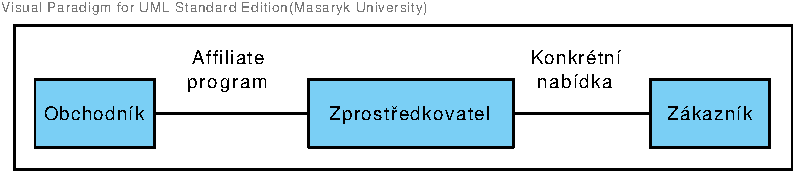
\includegraphics[]{vp/am-actors}}\hypertarget{idp54686880}{}%
            \label{idp54686880}
        }
        {{\caption[{Základní účastnické role affiliate 
marketingu}]{{{Základní účastnické role affiliate 
marketingu}}}\label{am-basic}}}
    \end{center}
\end{figure}

Proces interakce mezi jednotlivými aktéry je iniciován obchodníkem. Ten 
vytvoří tzv. affiliate program\index{affiliate program}, ve kterém 
specifikuje svou nabídku, kterou chce pomocí affiliate marketingu předložit 
zákazníkovi. Obvykle se jedná o~seznam produktů nebo služeb, spolu 
s~jejich parametry (popis, cena). Může jít však i o~nabídku v~podobě 
slevových kuponů, které nejsou vázány na konkrétní zboží, nebo obecnou 
inzerci (reklamní banner).

Nabídka od obchodníka je převzata partnerem. Tím může být, jak už bylo 
naznačeno, jakýkoli web disponující obsahem, díky němuž může těžit 
právě ze zobrazení reklamy. Přirozeným zprostředkovatelem jsou právě 
vydavatelské společnosti jako Future, které poskytují velké množství 
kvalitního obsahu a zároveň mají početnou a stabilní uživatelskou 
základnu, které je možné nabídku od obchodníků zobrazit. Ideální 
situace nastává, pokud je nabídka relevantní vůči kontextu obsahu, 
v~rámci kterého se objeví. V~takovém případě totiž nepochybně 
dochází ke zvýšení konverzního poměru, tedy množství uživatelů, 
které zobrazená reklama přiměje k~určité akci - typicky 
nákupu.\footnote{
    Jako příklad můžeme uvést technologický článek popisující 
vlasnosti nového mobilního telefonu, který se právě objevil na trhu. Obsah 
tohoto typu bude pravděpodobně vyhledáván zejména uživateli, kteří 
mají potenciálně zvýšený zájem o~koupi tohoto přístroje, a tedy i 
větší tendenci využít zobrazené nabídky tohoto produktu.
} Zároveň dochází 
k~situaci, ve které přestává být reklama vnímána jako reklama a díky 
kontextu okolního obsahu se sama stává 
obsahem.\footnote{
    V~návaznosti na předchozí příklad si můžeme představit, že pokud 
vydavatel zobrazí tři různé nabídky téhož produktu, spolu s~cenovým 
srovnáním, dává tak čtenáři článku kromě odborného názoru na 
samotný produkt i základní analýzu toho, kde a za jakou cenu je produkt 
možno zakoupit.
} V~takovém případě má 
vhodně zvolený affiliate program kromě pozitivního vlivu na příjmy 
vydavatelské společnosti také pozitivní vliv na spokojenost uživatelů, 
nebo minimálně na redukci jejich nespokojenosti s~nutností konzumace reklamy.

Posledním článkem nezbytným k~úspěšnému provozování affiliate 
marketingu je samotný uživatel. Ten se stává konzumentem nabídky a 
v~případě úspěšné konverze provádí nákupní rozhodnutí, díky 
němuž profitují všechny zúčastněné strany (win-win-win model).

% ------------------------   
% Section 
\section{Princip fungování}
\label{idp54697120}\hypertarget{idp54697120}{}%

Jelikož affiliate marketing je záležitostí internetových obchodů a 
webových poskytovatelů obsahu, je užitečné se zaměřit i na technickou 
stránku celého procesu interakce mezi jednotlivými aktéry popsanými 
v~kapitole \hyperlink{chap-roles}{{\ref{chap-roles}}}.
\subsection{Unikátní identifikátory}
\label{idp54699168}\hypertarget{idp54699168}{}%

Pro fungování affiliate marketingu je nejzásadnější existence 
unikátních kódů, pomocí nichž je možné identifikovat všechny 
konkrétní účastníky celého procesu. V~angličtině se tyto 
identifikátory označují pojmem {\em{tracking codes}}\index{tracking code}.

Jak bylo popsáno v~předchozí kapitole, prvním krokem je předání nabídky 
od obchodníka zprostředkovateli. V~tuto chvíli můžeme zjednodušit a pod 
nabídkou si představit konkrétní produkt, prodávaný v~e-shopu 
obchodníka. Zprostředkovatel (affiliate) dostane od obchodníka speciálně 
upravená data, jež obsahují právě unikátní kód identifikující daného 
zprostředkovatele. Tento identifikátor je obvykle součástí URL adresy. 
Zprostředkovatel data interpretuje a podle svého uvážení je vhodným 
způsobem zobrazí na své stránce. Ve chvíli, kdy čtenář obsahu nabídky 
využije, je přesměrován na stránku obchodníka. Zároveň je však tímto 
přesměrováním přenesen i identifikátor a obchodník tak může dohledat, 
od kterého affiliate partnera daný zákazník přišel.
\subsection{Provize}
\label{idp54704384}\hypertarget{idp54704384}{}%

Pravidla affiliate marketingu obvykle (narozdíl od klasické inzerce) 
neurčují, jakým způsobem má být nabídka zobrazena. Důvodem k~tomu je 
fakt, že inzerent (tedy obchodník) zprostředkovateli neplatí za zobrazení 
(jako u~klascké inzerce), a dokonce obvykle ani za kliknutí (tedy 
nasměrování uživatele na stránky obchodníka), jako je tomu u~systémů 
pay per click. \cite{marketing-performance}{} Zprostředkovateli je vyplacena 
provize na základě uskutečněných objednávek (nákupů), které 
uživatelé jím nasměrovaní do e-shopu obchodníka realizují. Výše 
provize je obvykle určena fixní procentní sazbou z~částky, kterou 
uživatel v~e-shopu utratí; obvykle se pohybuje mezi 2 a 10 \%.

V~některých případech může být výše provize fixní, jindy je vyplacena 
určitá částka i za každého příchozího zákazníka, ačkoli 
neuskuteční žádnou nákupní akci. Tyto modely jsou ale ve světě 
affiliate marketingu méně obvyklé.
\subsection{Odložené rozhodnutí o~nákupu}
\label{chap-odlozene-rozhodnuti}\hypertarget{chap-odlozene-rozhodnuti}{}%

Výše popsaný systém provizí se zdá být na první pohled spravedlivý. 
Nákupní chování ale není obvykle takto přímočaré. I~v~případě, že 
zákazník využije nabídky od zprostředkovatele, dostane se na stránky 
e-shopu a má zájem si daný prodkut koupit, obvykle neprovede nákup 
okamžitě. \cite{consumer-behavior}{} Ve hře je několik faktorů. Někteří 
zákazníci se potřebují před nákupem poradit s~autoritou, jiní prostě 
jen potřebují určitý čas, než rozhodnutí udělají. 
\cite{internet-marketing-strategy}{}

Dalším případem, kdy je rozhodnutí o~nákupu odkládáno, specifické pro 
svět webového marketingu, je existence slevových voucherů\index{slevový 
kupon}. Existují specializované servery, které nabízí velké množství 
slevových kuponů a kódů, které mohou zákazníci 
využít.\footnote{
    Velmi známým příkladem ve Velké Británii je server 
{\textless}\url{http://www.vouchercodes.com}{\textgreater}.
} Často jsou i tyto 
kupóny předmětem affiliate marketingu a pomocí unikátních 
identifikátorů z~nich provozovatelé těchto systémů získávají provizi 
stejným způsobem, jako klasičtí zprostředkovatelé.

Podstatou vyplácení provize, a potažmo celého affiliate marketingu, je 
ovšem odměna za přivedení zákazníka, resp. napomožení učinění 
nákupního rozhodnutí. Cílem všech zúčastněných stran je tedy 
maximální možné očištění o~zmíněné vlivy, které by vedly 
k~výraznému snížení provizí a tedy i nižší ochotě zprostředkovatelů 
na affiliate programech spolupracovat.
\subsection{Cookies}
\label{idp54716384}\hypertarget{idp54716384}{}%

Řešením problému popsaného v~předchozí sekci je vytvoření jakési 
\glqq paměti\textquotedblleft{} e-shopu, díky níž by byl schopen znovu 
identifikovat zákazníka, který na e-shop přišel skrze zprostředkovatele 
affiliate programu, neučinil nákupní rozhodnutí, ale následně se vrátil 
(tentokrát už ovšem ne nutně přes affiliate odkaz obsahující 
identifikátor daného zprostředkovatele) a nákup provedl.

Implementace této \glqq paměti\textquotedblleft{} je díky technologiím 
používaným na webu velmi přímočará díky použití tzv. cookies. Cookie 
je obyčejný soubor uložený v~klientském zařízení, tedy typicky 
počítači nebo tabletu s~webovým prohlížečem, sloužícím právě jako 
jakási \glqq paměť\textquotedblleft{} pro webové stránky. 
\cite{rfc-cookie}{} Při první návštěvě e-shopu skrze affiliate odkaz je 
do cookie uložen identifikátor zprostředkovatele. Pokud je z~téhož 
zařízení učiněn nákup, e-shop je díky cookie schopen rozpoznat, že se 
zákazník do internetového obchodu dostal právě přes affiliate partnera a 
podle toho vyplatí provizi.

Cookies v~affiliate marketingu dokonce většinou nejsou specifické ani pro 
konkrétní produkt. Pokud se tedy zákazník dostane do e-shopu s~elektronikou 
díky odkazu propagujícímu chytrý telefon, ale nakonec si koupí televizi, 
je zprostředkovateli vyplacena provize v~podobě procentuální sazby z~ceny 
koupené televize.

Aby byla zachována silná korelace mezi přivedením zákazníka 
prostřednictvím zprostředkovatele a nákupním rozhodnutím, je nutné dobu 
existence cookie časově omezit. Po určité době je tedy \glqq 
paměť\textquotedblleft{} e-shopu vynulována a pro přiznání provize je 
nutné, aby zákazník znovu využil affiliate odkaz. Tato doba se liší podle 
povahy a především velikosti internetového obchodu. Typicky je to 30 dní, 
ale například největší světový e-shop Amazon má životnost cookie 
pouhých 24 hodin. \cite{amazon-cookie}{} Zdůvodnění je poměrně logické. 
Lidé na Amazonu nakupují tak často, že připisování nákupu provedeného 
déle než 24 hodin po prokliknutí affiliate odkazu by místo pozitivního 
efektu zpřesnění přineslo více nepřesností v~podobě uznání provize i 
za nákupy, které zprostředkovatel díky affiliate programu neměl šanci 
nijak ovlivnit.\footnote{
    Zajímavým zlepšením tohoto problému by nepochybně bylo vytvoření 
unikátních cookies pro konkrétní produkt. Lze odůvodněně předpokládat, 
že v~takovém případě by bylo možné životnost cookies rapidně 
prodloužit, aniž by došlo k~výraznějšímu zkreslení v~podobě nákupů 
nemajícíh nic společného s~původní nabídkou affiliate programu. 
Evidentně je ale implementační náročnost na straně e-shopu natolik 
složitá, resp. neefektivní, že žádný z~velkých internetových obchodů 
podobnou taktiku zatím nezvolil.}

Podobně jako expiraci cookie je nutné zařídit i situaci, ve které 
uživatel využije několik affiliate odkazů od různých zprostředkovatelů, 
vedoucích do téhož e-shopu. Nedává smysl, aby e-shop platil provizi 
každému z~nich. V~tomto případě platí pravidlo, že poslední bere vše, 
tedy provize je připsána zprostředkovateli, na jehož odkaz uživatel 
kliknul v~pořadí jako poslední.

% ------------------------   
% Section 
\section{Affiliate sítě}
\label{chap-ans}\hypertarget{chap-ans}{}%

V~kapitole \hyperlink{chap-roles}{{\ref{chap-roles}}} byly popsány tři role 
figurující v~procesu fungování affiliate marketingu: obchodník, affiliate 
a zákazník. V~této části je schéma rozšířeno o~dalšího účastníka, 
kterým je affiliate síť.
\subsection{Problém přímé interakce}
\label{idp54730672}\hypertarget{idp54730672}{}%

V~modelu v~tuto chvíli nebudeme uvažovat zákazníka. Ten je sice 
důležitý, ale hraje ve struktuře pouze roli konzumenta obsahu a při 
rozšíření o~affiliate síť se jeho role nemění. Situace je tedy taková, 
že na jedné straně e-shopy uveřejňují svou nabídku a snaží se 
přesvědčit vydavatelské společnosti, aby jejich produkty zobrazovaly 
u~recenzí. Na straně druhé se vydavatelské společnosti snaží získat 
nabídky pro své e-magazíny. Schéma zobrazující příklad takových 
vztahů se jmény známými z~českého prostředí zobrazuje diagram 
\hyperlink{fig-an-m-to-n}{{\ref{fig-an-m-to-n}}}.

% figure ------------------------------------------------------
\begin{figure}[hbt]
    \hypertarget{fig-an-m-to-n}{}%
    \begin{center}

        {{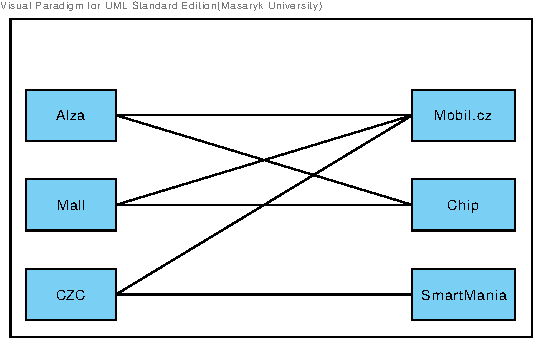
\includegraphics[]{vp/am-m-to-n}}\hypertarget{idp54735024}{}%
            \label{idp54735024}
        }
        {{\caption[{Přímá interakce mezi obchodníky a 
vydavateli}]{{{Přímá interakce mezi obchodníky a 
vydavateli}}}\label{fig-an-m-to-n}}}
    \end{center}
\end{figure}

Každý vztah mezi e-shopem a vydavatelem, vyjádřený v~diagramu čárou, 
musí být vyjednán zvlášť. A~to jak obchodní podmínky, tak zejména 
technická stránka celého procesu. Nabídka produktů může mít u~každého 
obchodníka jinou strukturu a může být dostupná rozdílnými způsoby (jako 
soubor na FTP serveru, přes REST rozhraní, \ldots). Stejně tak každý 
obchodník může mít jinak nastavenou výši provizí nebo frekvenci jejich 
vyplácení. Toto jsou jen příklady problémů, kterým jsou účastníci 
vystaveni ve velké míře při přímé komunikaci. Většinu těchto 
problémů řeší právě další účastník -- affiliate síť.
\subsection{Sjednocení komunikace}
\label{idp54738176}\hypertarget{idp54738176}{}%

Affiliate síť je třetí strana, která sama o~sobě není e-shopem (nemá 
vlastní nabídku produktů) a není ani vydavatelem, tedy nezobrazuje žádné 
nabídky zákazníkům. Affiliate síť funguje jako zprostředkovatel mezi 
obchodníky a affiliate partnery (tedy typicky vydavateli). Princip jejího 
fungování spočívá v~tom, že tvoří jakési odstínění pro obě strany. 
Agreguje nabídky jednotlivých obchodníků, zaznamenává jejich podmínky a 
ty potom v~jednotném a dobře definovaném formátu předává vydavatelům. 
Podobně transparentní je při zahrnutí affiliate sítě celý proces i pro 
e-shopy, které přestávají řešit separátně jednotlivé vydavatele. Pouze 
zveřejní svou nabídku v~rámci affiliate sítě, která za ně řeší 
komunikaci s~vydavateli a konkrétní technické řešení. Z~původního 
schématu M:N se tak ve skutečnosti stávají dvě skupiny s~kardinalitami M:1 
a 1:N. Jak je vidět z~diagramu 
\hyperlink{fig-am-m-to-n-with-an}{{\ref{fig-am-m-to-n-with-an}}}, množství 
nutných interakcí se snížilo z~kvadratického na lineární.

% figure ------------------------------------------------------
\begin{figure}[hbt]
    \hypertarget{fig-am-m-to-n-with-an}{}%
    \begin{center}

        {{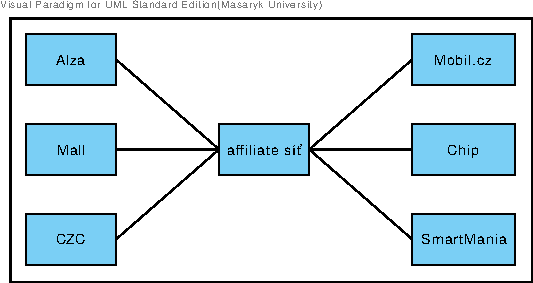
\includegraphics[]{vp/am-m-to-n-with-an}}\hypertarget{idp49338016}{}%
            \label{idp49338016}
        }
        {{\caption[{Interakce mezi obchodníky, affiliate sítí a 
vydavateli}]{{{Interakce mezi obchodníky, affiliate sítí a 
vydavateli}}}\label{fig-am-m-to-n-with-an}}}
    \end{center}
\end{figure}

\subsection{Důsledky využití affiliate sítě}
\label{idp49339328}\hypertarget{idp49339328}{}%

Využití affiliate sítě má několik důsledků. Zahrnutí třetí strany 
znamená, že obchodník nebo vydavatel musí za poskytnutou službu tuto 
stranu, tedy affiliate síť, kompenzovat. Existují dva obvyklé modely: 
rozdělení provize za prodej výrobku mezi síť a vydavatele, nebo přímé 
(paušální) zpoplatnění přístupu k~datům poskytovaným affiliate sítí.

Jednoznačně pozitivním důsledkem z~hlediska vydavatelské společnosti je 
sjednocení komunikačních kanálů a datových formátů. I~přesto, že 
různí obchodníci mohou mít jinak nastaveno například rozdělení 
produktů do kategorií nebo frekvenci vyplácení provizí, je úlohou 
affiliate sítě tyto rozdíly minimalizovat. Vydavatel tak může sledovat 
výši provize od všech obchodníků naráz v~administračním rozhraní 
affiliate sítě. Stejně tak samotná data jsou dostupná obvykle na jednom 
místě a v~jednotném formátu.

Samozřejmě neexistuje pouze jedna univerzální affiliate síť s~monopolem 
na veškerá data týkající se affiliate marketingu. Affiliate sítí je 
celá řada a zejména ve Velké Británii a v~USA jsou jejich služby 
vydavateli hojně využívány. Se vzrůstajícím počtem affiliate sítí 
přestává být zřetelná výhoda sjednocení komunikačních kanálů, 
zatímco nutnost sdílení příjmů zůstává. Evidentně se ale vydavatelům 
vyplácí využívání affiliate sítí. Komunikace s~deseti affiliate 
sítěmi je jednodušší než vlastní řešení pro každý z~několika 
stovek nebo tisíců e-shopů. Navíc často platí, že nabídky některých 
obchodníků nejsou dostupné jinak než prostřednictvím některé 
z~affiliate sítí -- vydavatelé tak nemají příliš na výběr.

Snížení počtu interakcí popsané v~předchozí sekci nezahrnuje jen 
komunikaci podmínek a získání nabídky obchodníka, ale figuruje i při 
nákupní akci samotného uživatele. Veškeré odkazy na nabídky produktů, 
které vydavatel přes affiliate síť získá, nevedou přímo do e-shopu, ale 
obsahují adresu affiliate sítě. Po kliknutí na nabídku je tedy uživatel 
přesměrován tam, affiliate síť požadavek zaznamená a přesměruje 
uživatele do e-shopu. Přestože návštěvník webu tento \glqq krok 
navíc\textquotedblleft{} téměře nepostřehne, pro princip fungování 
celého systému affiliate marketingu je velmi důležitý. Na webové stránce 
obchodníka je totiž zaznamenán pouze příchod z~affiliate sítě, takže 
veškeré provize jsou vypláceny pouze síti. Pokud tedy do určtitého 
e-shopu přes affiliate síť přicházejí zákazníci z~deseti 
vydavatelských portálů, obchodník počítá a vyplácí provizi pouze 
jednou, ve smyslu čáry interakce zobrazené v~diagramu 
\hyperlink{fig-am-m-to-n-with-an}{{\ref{fig-am-m-to-n-with-an}}}. Stejným 
způsobem jsou pak výsledky, jak finanční tak informační, předávány 
vydavateli v~agregované 
podobě.\footnote{
    Vydavatelé i obchodníci mají obvykle zájem být informováni o~tom, kam 
nebo odkud konkrétně jsou jejich uživatelé směrováni. Tento tzv. \glqq 
tracking\textquotedblleft{} je obvykle řešen na úrovni speciálního 
parametru v~URL adrese a neovlivní tak významněji popsané schéma.}

Posledním důsledkem využití affiliate sítí jako dalšího článku 
v~komunikačním řetězci je zpoždění, které může při předávání 
informací nastat. Kritické je zejména při aktualizaci nabídky 
jednotlivých obchodníků. Pokud se tedy obchodník rozhodne určitý produkt 
zlevnit, tuto informaci předá přes programové rozhraní nikoliv přímo 
vydavateli, ale affiliate síti. Obvykle trvá až 24 hodin, než je cena 
aktualizována a změna je tak dostupná vydavateli. Zejména u~obchodníků, 
kteří mění ceny velmi často (např. Amazon), se může jednat o~podstatný 
nedostatek. Z~toho důvodu jsou někdy k~dispozici tzv. \glqq delta 
soubory\textquotedblleft{}, které jsou aktualizovány častěji (např. jednou 
za hodinu) a obsahují pouze ty produkty, jejichž cena byla změněna.

% ------------------------   
% Section 
\section{Alternativní zajištění příjmu z~webového obsahu}
\label{idp54765360}\hypertarget{idp54765360}{}%

Kromě affiliate marketingu, kterým se tato práce zabývá, existuje mnoho 
dalších způsobů, jakými lze zajistit stabilní proud příjmů z~webového 
obsahu, resp. e-magazínů. V~této části jsou tyto alternativy zevrubně 
popsány a jejich fungování je porovnáno s~principy affiliate marketingu.
\subsection{Cost per impression}
\label{idp54767136}\hypertarget{idp54767136}{}%

Klasická online reklama je pravděpodobně jedním z~prvních typů 
internetového marketingu, který se na webu objevil. Ve svém základním 
modelu vychází z~principů reklamy, tak jak funguje v~tištěných médiích. 
Inzerent si objedná určité množství zobrazení své (dopředu vytvořené) 
reklamy, ať už se jedná o~reklamu čistě textovou nebo mající i grafickou 
podobu. Za každé zobrazení reklamy pak zaplatí určitou, zpravidla fixní 
částku. Tento model se nazývá anglickým termínem {\em{Cost per 
impression}}, často zkracovaným jako CPI\index{cost per impression}.

V~oblasti webového marketingu jde pravděpodobně o~metodu affiliate 
marketingu nejvíce vzdálenou, protože není vázána na žádnou akci ze 
strany uživatele. Ten si často reklamy ani nemusí všimnout, cena za 
zobrazení tak bývá obvykle stanovena poměrně nízko a téměř nikdy není 
vázána kontextově na konkrétní produkt, který je reklamním bannerem 
inzerován.
\subsection{Pay per click}
\label{idp54771328}\hypertarget{idp54771328}{}%

O~něco bližším modelem inzerce v~prostředí webu je metoda {\em{Pay per 
click}} (PPC)\index{pay per click}. Stejně jako v~případě CPI je založena 
na zobrazení předem vytvořené reklamy v~textové nebo grafické podobě. 
Inzerent ovšem neplatí za zobrazení reklamy, ale, jak už napovídá název, 
pouze za proklik. Tato metoda sice koreluje s~tržbami realizovanými díky 
inzerci více než CPI, nicméně stále pro obchodníka nepředstavuje jistou 
investici. I~velké množství prokliků a razantní zvýšení návštěvnosti 
nemusí znamenat zvýšení prodejů. \cite{am-impact}{}

Metoda PPC bývá často využívána společnostmi provozujícími 
vyhledávací stroje.\footnote{
    Společnost Google provozuje systém AdWords, český Seznam disponuje 
obdobnou službou Sklik.}
U~výsledků 
vyhledávání je tak kromě samotných reálných výsledků založených na 
porovnávání obsahu webových dokumentů obvykle zařazeno několik \glqq 
sponzorovaných\textquotedblleft{} položek. \cite{customers-now}{} Ty jsou 
většinou vizuálně odlišeny, nicméně ne natolik, aby je uživatel 
nepovažoval za relevantní výsledek vyhledávání. Tento fakt umocňuje 
skutečnost, že PPC reklama je obvykle kontextově koherentní s~ostatními 
výsledky vyhledávání.

Princip objednávání je závislý na konkrétním systému. Obecně (a 
s~určitou mírou zjednodušení) lze ovšem říct, že zařazení reklamy do 
výsledků vyhledávání pro určité klíčové slovo se řídí principem 
aukce. Pro dané klíčové slovo tedy existuje několik málo pozic, které 
obsadí inzerenti, jež jsou ochotni zaplatit za proklik nejvyšší částku. 
\cite{razeni-inzeratu-seznam}{}

Hranice mezi modelem PPC a affiliate marketingem je často neostrá a oba typy 
marketingu se vzájemně prolínají. Existují affiliate programy, kde 
obchodník (resp. obecně inzerent) platí pouze za proklik, a de facto se tedy 
jedná o~model PPC. Stejně tak například PPC program Sklik, provozovaný 
českým Seznamem, nabízí Partnerský program, v~rámci kterého mohou 
partneři (tedy affiliates) na své stránky umisťovat a graficky upravovat 
reklamní bannery. \cite{partnersky-program-seznam}{} Ve skutečnosti tedy 
takový program splňuje základní kritéria affiliate marketingu.
\subsection{Placený obsah}
\label{idp54781184}\hypertarget{idp54781184}{}%

Poměrně odlišným obchodním modelem oproti doposud zmíněným metodám je 
přímá platba za obsah. Proces, který je zcela běžný v~prostředí 
klasických tištěných médií, se jen velmi těžko uplatňuje na webu.

Zpoplatněný obsah na webu lze v~zásadě rozdělit do tří skupin. První 
skupinou je elektronický ekvivalent tištěného obsahu, ať už v~podobě 
elektronické knihy nebo možnosti stáhnout si elektronickou verzi 
předplaceného magazínu. Do druhé skupiny lze zařadit vysoce 
specializované a odborné portály, které nemají tištěný ekvivalent, 
nicméně uživatelé jsou ochotni za přístup k~nim platit. Obě dvě 
zmíněné skupiny mají už v~oblasti internetu poměrně silnou tradici, 
ověřené obchodní modely a stabilní zákaznickou základnu. Kromě 
elektronických knih mezi ně lze zařadit i elektronické verze odborných 
akademických časopisů a vědecké databáze.

Zcela odlišnou skupinou jsou ovšem klasické elektronické magazíny, 
jejichž čtenáři zpravidla nejsou zvyklí za přístup k~nim platit. Může 
se jednat o~spcializované servery, ale i zpravodajské portály. Vzhledem 
k~tomu, že na webu existuje obrovské množství podobných produktů, je 
poměrně těžké naráz zpoplatnit přístup k~obsahu e-magazínu, protože 
uživatelé mohou snadno přejít k~používání konkurenčního produktu.

Přesto se některé velké zpravodajské severy o~obchodní model založený 
na přímé platbě za přístup k~obsahu snaží. Typicky to vede k~poměrně 
razantnímu poklesu návštěvnosti, jehož míru je navíc velmi obtížné 
dopředu odhadnout. Například elektronická verze The Times po zpoplatnění 
přišla o~dvě třetiny návštěvníků, ovšem očekával se pokles až 90 
\%. \cite{times-reuters}{} Zatím také není úplně jasné, na jaké cenové 
hladině by se měl placený přístup k~webovým magazínům nacházet.

% -------------------------------------------------------------
% Chapter Specifika e-commerce software 
% ------------------------------------------------------------- MainMatter
\cleardoublepage\chapter{Specifika e-commerce software}
\label{chap-ecom-soft}\hypertarget{chap-ecom-soft}{}%

Webové vydavatelské společnosti se pohybují na rozhraní mezi vytvářením 
produktu a poskytováním služby. Stejně jako klasické magazíny, i obsah 
zpravodajského webu lze označit za produkt. Má sice elektronickou podobu, 
ale na obrazovce počítače, tabletu nebo telefonu je zobrazen velmi podobně 
jako klasický papírový magazín, o~jehož produktové povaze není pochyb.

Na druhou stranu e-magazín (a obecně jakýkoli typ webových dokumentů) 
splňuje většinu základních charakteristik služeb, jako je nehmotnost a 
nemožnost vlastnictví ze strany zákazníka. Aspekt služby je pak ještě 
umocněn v~případě, že jakákoli část webu je interaktivní. 
Zákazníkovi je pak místo prosté konzumace obsahu (tedy jakéhosi 
používání teoretického produktu) zprostředkovávána služba -- 
většinou informačního charakteru. Může se jednat o~internetový jízdní 
řád, portál zprostředkovávající pracovní nabídky anebo e-commerce 
platformu poskytující cenové srovnání a možnost nákupu různých 
produktů.

Právě v~oblasti e-commerce se nachází většina řešení využívajících 
affiliate marketing. Z~pohledu vydavatele se široký pojem e-commerce omezuje 
na poskytnutí informace o~nabídce a nasměrování zákazníka do 
internetového obchodu. Samotné zakoupení produktu nebo služby už není 
z~pohledu provozovatele e-magazínu součástí tohoto procesu. Jedinou 
klíčovou informací je výše konverzního poměru -- tedy poměr 
uživatelů, kteří nakonec nákup skutečně provedou, vůči celkovému 
objemu přesměrovanému do internetového obchodu.

Tato kapitola se věnuje principům tvorby e-commerce software. V první části
je popsáno, jakým způsobem probíhá proces nákupního chování a jakými
aspekty je finální rozhodnutí ovlivněno. Nástroje affiliate marketingu
by měly tyto principy co nejlépe využívat. V~druhé části této kapitoly
je rozebírán způsob vývoje a inovace softwarového produktu, zejména webového typu.

% ------------------------   
% Section 
\section{Proces nákupního rozhodování}
\label{chap-nakupni-rozhodovani}\hypertarget{chap-nakupni-rozhodovani}{}%

Z~pohledu marketingu obecně je klíčové porozumění nákupnímu chování 
zákazníka. Stejně je tomu i v~případě webové platformy a affiliate 
marketingu. Jak bylo zmíněno v~úvodu této kapitoly, rozhodující je 
nasměrování zákazníka do internetového obchodu. A~rovněž zde platí 
základní modely nákupního chování a rozhodování, které byly původně 
vytvořeny pro analýzu klasického nákupu. Internet je totiž pouze 
prostředím, ve kterém se zákazník rozhoduje, nikoliv předmětem 
samotného rozhodování. Tím zůstává samotný akt nákupu klasického 
produktu, například spotřební elektroniky, jako je tomu v~případě 
e-magazínu TechRadar.
\subsection{Model DAGMAR\index{DAGMAR}}
\label{chap-dagmar}\hypertarget{chap-dagmar}{}%

Tato práce vychází ze dvou modelů hierarchie účinků nákupního 
rozhodování. Prvním z~nich je koncept, jež představil pod názvem \glqq 
Defining Advertising Goals for Measured Advertising Results\textquotedblleft{} 
v~roce 1961 Russel H. Colley. \cite{dagmar}{} Tento model v~základní podobě 
popisuje sekvenci, kterou prochází potenciální zákazník při procesu 
nákupního rozhodování. Prvním krokem je získání povědomí o~existenci 
produktu (awareness). Pokud zákazník získá dostatek informací (fáze 
comprehension), rozhodne se k~nákupu (conviction). Samotný akt nákupu je 
poslední fází (action). Celý proces zobrazuje diagram 
\hyperlink{fig-dagmar}{{\ref{fig-dagmar}}}.

% figure ------------------------------------------------------
\begin{figure}[hbt]
    \hypertarget{fig-dagmar}{}%
    \begin{center}

        {{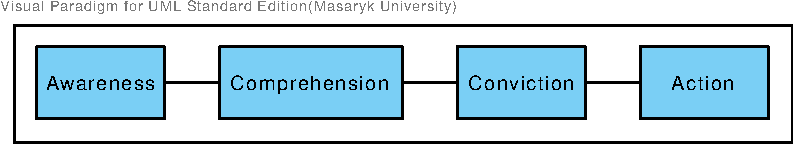
\includegraphics[]{vp/dagmar}}\hypertarget{idp54801136}{}%
            \label{idp54801136}
        }
        {{\caption[{Hierarchie modelu DAGMAR}]{{{Hierarchie modelu 
DAGMAR}}}\label{fig-dagmar}}}
    \end{center}
\end{figure}

Z~pohledu vydavatele, který se pomocí nástrojů affiliate marketingu snaží 
nasměrovat své uživatele k~internetovým obchodníkům, jsou klíčové 
zejména prostřední dvě fáze. Obsahem, tedy zejména recenzemi spotřební 
elektroniky, zprostředkovává čtenáři velké množství odborných 
informací o~produktu, především z~technického úhlu pohledu. Pokud je 
recenze pozitivní, může čtenáře přesvědčit o~nákupu.

E-magazín jako TechRadar hraje určitou roli i v~první fázi, tedy 
informování zákazníka o~existenci nového produktu, vytvoření 
základního povědomí. Tato úloha ovšem není zdaleka tak silná, jak by se 
mohlo zdát. Jelikož se nejedná o~zpravodajský server, většinu 
návštěvníků tvoří uživatelé, kteří jsou už dopředu velmi zběžně 
obeznámeni s~tím, jaké produkty na trhu existují. E-magazín jim pak 
především pomáhá upřesnit a rozšířit si informace o~těchto produktech.
\subsection{Matice FCB\index{FCB}}
\label{idp54804464}\hypertarget{idp54804464}{}%

Druhým modelem, ze kterého tato práce vychází, je matice Foote Cone 
Belding (FCB). \cite{fcb-how-advertising-works}{} Ten narozdíl od 
předchozího teoretického konceptu neurčuje sekvence, které vedou 
k~nákupu, ale rozděluje doménu nakupovaných výrobků (a služeb) do čtyř 
oblastí určených kombinací dvou binárních 
proměnných.\footnote{
    Proměnné jsou ve skutečnosti binární pouze pro účely rozdělení do 
čtyř oblastí. Ve skutečnosti model počítá i s~\glqq 
fuzzy\textquotedblleft{} hodnotami, takže na škále lze určovat i \glqq 
vzdálenost\textquotedblleft{} od opačného pólu. Spíše než aby 
přoměnná nabývala jedné ze dvou diskrétních hodnot se tedy pohybuje na 
spojité škále.}

První proměnnou je stupeň zaujetí při rozhodovacím procesu. V~FCB modelu 
vysoký stupeň zaujetí charakterizuje vysokou míru motivace v~rozhodovacím 
procesu. Typicky je tento přístup charakteristický pro dražší výrobky a 
služby, které zákazník nekupuje často. Naopak výrobky denní spotřeby se 
v~FCB matici nacházejí v~oblasti nízkého stupně zaujetí. Rozhodovací 
proces je zde buď velmi zběžný a povrchní, nebo již proběhl a výrobek 
je nakupován opakovanně -- nákup se stává rutinním chováním. Vysoký 
stupeň zaujetí je v~FCB matici obvykle zobrazován v~horní polovině, 
nízký stupeň zaujetí ve spodní.

Druhou proměnnou, v~matici FCB obvykle znázorněnou na pravo-levé ose, je 
míra racionality zapojená do rozhodování. Levá část FCB matice zobrazuje 
takové výrobky a služby, při jejichž nákupu zákazník v~rámci 
rozhodovacího procesu více přemýšlí a zkoumá informace. Pravá část 
matice zahrnuje naopak chování, které je více impulzivní. Zákazník se 
u~těchto výrobků a služeb rozhoduje více \glqq 
instinktivně\textquotedblleft{} a nezkoumá fakta a podrobnosti.

FCB matici s~příklady typických produktů zobrazuje obrázek 
\hyperlink{fig-fcb}{{\ref{fig-fcb}}}. 

% figure ------------------------------------------------------
\begin{figure}[hbt]
    \hypertarget{fig-fcb}{}%
    \begin{center}

        {{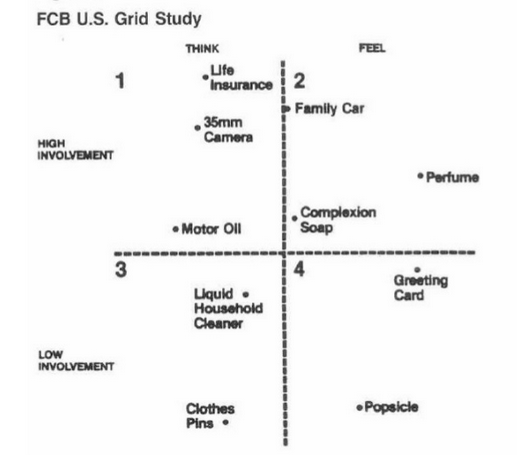
\includegraphics[width=300px]{img/fcb}}\hypertarget{idp54815600}{}%
            \label{idp54815600}
        }
        {{\caption[{Příklad matice FCB}]{{{Příklad matice FCB \cite{fcb-how-advertising-works-slideshare}{}}}}\label{fig-fcb}}}
    \end{center}
\end{figure}

Pořízení spotřební elektroniky, kterou se z~pohledu e-magazínu TechRadar 
tato práce zabývá, lze obvykle zařadit do prvního kvadrantu (vlevo 
nahoře). Nákupní rozhodnutí v~takovém případě charakterizuje vysoký 
stupeň zaujetí. Zároveň obvykle spadá do oblasti racionálního 
zhodnocení existujících možností. Uživatelé často pročítají recenze 
a porovnávají různé nabídky podobných nebo stejných produktů 
v~různých obchodech.\footnote{
    Tato domněnka je ověřena i v~rámci dotazníkového šetření 
v~kapitole \hyperlink{chap-vyzkum}{{\ref{chap-vyzkum}}} a ukazuje se jako 
správná.}
\subsection{Role affiliate marketingu v~nákupním procesu}
\label{chap-role-am-v-nakupnim-procesu}\hypertarget{chap-role-am-v-nakupnim-proc
esu}{}%

Využití znalosti o~nákupním rozhodování je užitečné pro správný 
návrh provádění affiliate marketingu. Cílem vydavatelské společnosti je 
poskytnutí dodatečných informací o~produktu, který zákazníka zajímá. 
Jak bylo zmíněno v~sekci \hyperlink{chap-dagmar}{{\ref{chap-dagmar}}}, 
prvním krokem je vytvoření základního povědomí o~produktu. Většina 
čtenářů recenzí e-magazínu už takovou znalost má -- chtějí pro 
konkrétní produkt dohledat dodatečné informace. Přesto může být 
užitečné vytvářet i rozcestníky a informační články o~nových 
produktech, na které pak navazují recenze. Čtenář tak může i při 
dohledávání informací o~produktu A~narazit na jiný produkt B, pro který 
se nakonec rozhodne.

Z~pohledu modelu DAGMAR je ale potřeba soustředit se především na kroky 
\glqq Comprehension\textquotedblleft{} a \glqq Conviction\textquotedblleft{}. 
Vydavatel e-magazínu by měl být schopen čtenáři zprostředkovat takové 
množství informací, aby si byl schopen udělat dostatečnou představu 
o~nabídce na trhu a vlastnostech konkrétních produktů. To znamená jednak 
obsahovou úplnost recenzí v~e-magazínu, a také přímou aplikaci affiliate 
marketingu v~podobě odkazů do internetových obchodů. V~rámci úplnosti 
informací může být pro zákazníka užitečné vidět nejen vlastnosti 
produktu a jeho ceny, ale i další atributy jako je dodací lhůta, 
speciální nabídky nebo slevové kupony. Všechny tyto faktory zkoumány 
v~praktické části práce -- kapitole 
\hyperlink{chap-aplikace-am}{{\ref{chap-aplikace-am}}}.

Jedním z~nejpalčivějších problémů, které e-magazíny v~oblasti 
affiliate marketingu řeší, je tzv. \glqq poslední krok\textquotedblleft{}. 
Jak bylo popsáno v~kapitole \hyperlink{chap-am}{{\ref{chap-am}}}, provize je 
vyplacena zprostředkovateli (vydavateli e-magazínu) jen v~tom případě, že 
je zákazník do e-shopu nasměrován přímo z~daného e-magazínu, tedy 
učiní zde zpravidla poslední rozhodující krok před nákupem. Pokud forma 
affiliate marketingu ve webovém magazínu nepostihuje všechny aspekty 
nákupního rozhodování, může uživatel v~zájmu úplnosti informací 
využít ještě další server, například se slevovými kupony, a poslední 
krok pak učiní z~něj. Tím se vydavatel e-magazínu připravuje o~provizi, 
ačkoliv mohly ve skutečnosti o~nákupu zákazníka přesvědčit právě jeho 
informace.

Vysoký stupeň zaujetí v~nákupním procesu, spolu v~kombinaci 
s~racionálním rozhodováním, se často vyznačuje poměrně dlouhým 
procesem hodnocení existujících možností. Ačkoli je potenciální 
zákazník přesvědčen o~koupi produktu, poměrně dlouho mu může trvat 
shromažďování potřebných informací, výběr konkrétního modelu a volba 
obchodu. Implementace affiliate marketingu naštěstí s~tímto přístupem 
částečně počítá a (jak bylo popsáno v~kapitole 
\hyperlink{chap-odlozene-rozhodnuti}{{\ref{chap-odlozene-rozhodnuti}}}) 
umožňuje započítání konverze i v~případě, že zákazník nákupní 
rozhodnutí neučiní ihned.

Ne všechny produkty inzerované v~rámci affiliate marketingu ale nutně 
spadají do první kategorie modelu FCB. Pokud se jedná například o~doplňky 
nebo příslušenství, u~kterých hraje velkou roli vzhled a jsou obecně 
méně nákladné, zákazníci budou mít větší tendenci provádět nákup 
impulzivně a nad rozhodnutím nestráví tolik času. V~tomto případě 
může být vhodné přesvědčit zákazníka o~nákupu časovým omezením 
nabídky, exkluzivní slevou nebo jiným stimulem, který přiměje uživatele 
provést akci bez většího otálení.

% ------------------------   
% Section 
\section{Vývoj a inovace softwarového produktu}
\label{sect-vyvoj-a-inovace}\hypertarget{sect-vyvoj-a-inovace}{}%

Ačkoliv software, obzvláště na webu, postrádá některé klasické aspekty 
hmotných produktů, princip vývoje a inovací je velmi podobný. Narozdíl od 
klasických výrobků je vývoj a inovace software klíčovou a často velmi 
zdlouhavou a nákladnou fází, která do značné míry nahrazuje fázi 
výroby. Jednou vytvořený software, opět zejména na webu, není potřeba 
znovu \glqq vyrábět\textquotedblleft{}. Naopak se zde objevují nové fáze 
jako je nasazení a údržba.

Webový e-magazín, stejně jako jiný obsah na webu, je specifický tím, že 
uživatel je neustále v~kontaktu s~poskytovatelem služby -- tedy tvůrcem 
webu. Pokud je vyvinuta nová verze produktu, je pouze na uvážení 
provozovatele, zda tuto novou verzi uvolní pro všechny uživatele. Ti tak 
většinou nemají na výběr, zda chtějí používat novou nebo starou verzi 
produktu, a po určité době testování nové verze je ta stará obvykle 
znepřístupněna. Příkladem můžou být webové portály od Twitteru až po 
Informační systém Masarykovy univerzity. 
\cite{twitter-redesign, is-mu-redesign}{}

Výsledky inovace a zlepšování produktu je tak možné sledovat 
s~okamžitým efektem. Pokud je procesem inovace odstraněn nějaký 
nedostatek, ať už bezpečnostní nebo fukční, s~nasazením nové verze se 
tato záplata okamžitě automaticky vztahuje na všechny 
uživatele.\footnote{
    Zde je určitý rozdíl oproti klasickému \glqq 
krabicovému\textquotedblleft{} software, u~kterého často uživatelé, ať 
už vědomě nebo nevědomě, odmítají instalovat aktualizace a tím 
přijmout inovaci, kterou výrobce nabízí.}
\subsection{Zachycení potřeb uživatelů}
\label{idp54840032}\hypertarget{idp54840032}{}%

Základním pravidlem úspěšné inovace není vytvoření perfektního 
produktu, ale řešení, které maximálně uspokojí potřeby zákazníků. 
\cite{advertising-creative}{} Stejné pravidlo platí i v~případě webového 
e-magazínu, resp. jeho části zaměřující se na umožnění jednoduchého 
nákupu produktů skrze prostředky affiliate marketingu. Cílem je tedy 
v~maximální možné míře zachytit požadavky a očekávání uživatelů.

Softwarový produkt (resp. služba) webového typu s~sebou nese v~oblasti 
zachycení uživatelských požadavků a očekávání několik úskalí. 
Uživatelé v~drtivé většině mají již nějaké zkušenosti s~webovými 
aplikacemi a tedy nastavenou určitou základní úroveň očekávání. Jednak 
je poměrně obtížné tuto základní úroveň očekávání aproximovat, 
neboť má obvykle velký rozptyl a zároveň jde o~\glqq 
implicitní\textquotedblleft{} očekávání. Uživatelé (a často ani 
tvůrci) si tedy neuvědomují doopravdy všechna očekávání, což se týká 
funkčních i nefunkčních požadavků. Jako příklad můžeme uvést dobu 
odezvy u~webové stránky v~řádu stovek milisekund, která je v~dnešní 
době považována za standard, ovšem stále musí být brána v~úvahu při 
tvorbě systému.\footnote{
    Doba odezvy je jako příklad uvedena záměrně. Základním rysem 
affiliate systémů je zpracovávání velkého množství dat, která jsou 
poskytována třetí stranou (obvykle affiliate sítěmi). Technicky je 
prakticky nemožné provádět zpracování dat až v~reakci na uživatelský 
požadavek, aniž by se zároveň zvýšila doba odezvy minimálně na jednotky 
sekund. Toto je typický příklad požadavku, který uživatelé ani tvůrci 
implicitně neuvažují, ale je potřeba s~ním při návrhu systému počítat.}

Mnohem efektivnější může být místo zkoumání absolutních 
hodnot\footnote{
    Absolutní hodnotou je myšlen jak předmět očekávání (např. 
zmíněná doba odezvy), tak jeho kvantitativní či kvalitativní hodnota (ve 
zmíněném případě např. \glqq méně než 100 ms\textquotedblleft{}).}
očekávání zjistit 
rozdíl mezi očekávanou službou a službou skutečně poskytnutou - tzv. gap 
skór, který určuje výslednou spokojenost s~poskytnutou službou. 
\cite{spokojenost-lukasova}{} V~takovém případě není zkoumáno 
očekávání samotné, ale pouze výše naplnění a odchylka od určité 
základní úrovně. Hlavní nevýhodou je pak fakt, že tato základní 
úroveň je prakticky nezjistitelná a v~rámci různých uživatelů může 
být výrazně odlišná. Někteří pokročilejší uživatelé mohou 
považovat za samozřejmost absolutní interaktivitu webové 
aplikace,\footnote{
    Webová aplikace načtená celá v~prohlížeči, s~prakticky nulovou dobou 
odezvy, tzv. \glqq single page application\textquotedblleft{}.}
u~jiných může být 
základní očekávání omezeno na prosté zobrazení základních informací. 
Problémem při použití gap skóru je ovšem nutnost nechat uživatele 
službu vyzkoušet. To může být problematické v~případě vývoje nového 
produktu či služby, případně pokud je prováděna významnější inovace. 
V~takovém případě je řešením iterativní vyvoj a prototypování. 
V~úvodní fázi vývoje produktu je vytvořen prototyp, na základě kterého 
je zjištěna míra naplnění očekávání ze strany uživatelů. 
V~závislosti na uživatelském testování a výsledcích této analýzy je 
prototyp zdokonalen (případně je vytvořen prototyp zcela nový). Celý 
postup je iterován, dokud uživatelské testování nepotvrdí přijatelnou 
úroveň.

Stinnou stránkou zmíněného postupu je jeho časová a finanční 
náročnost. Kromě vytváření samotného prototypu stojí samotné 
uživatelské testování velké množství času školených pracovníků, a 
samozřejmě také testovaných uživatelů.

Jednodušším způsobem je tedy zjištění obecně platných vzorců 
chování,\footnote{
    Jedná se zejména o~nákupní chování, ale obecně lze takto postihnou 
většinu aspektů vyvíjené služby.}
kterými se uživatelé 
řídí. Na základě těchto vzorců jsou vytvořena základní pravidla, 
podle který se návrh produktu nebo služby řídí. V~případě affiliate 
marketingu jde o~znalost toho, jakým způsobem se návštěvník webu 
rozhoduje o~nákupu, například zda je ve většině případů rozhodnut 
o~koupi produktu určitého typu a vybírá konkrétní model. Anebo jestli má 
uživatel už vybraný i konkrétní model a hledá jen konkrétní obchod. 
Následně pak kritéria, na základě kterých vybírá -- zda je 
nejdůležitější cena, jaký vliv má na rozhodnutí výše poštovného a 
doručovací lhůta a podobně. Právě na ověření těchto obecnějších 
konceptů je zaměřena praktická část této práce.

Posledním aspektem vývoje projektu v~oblasti affiliate marketingu ve velké 
vydavatelské společnosti, který je potřeba zmínit, je fakt, že 
uživatelé nevystupují v~roli zákazníků. Návštěvníci webu 
(uživatelé) přímo nespecifikují své požadavky a dokonce ani za službu 
přímo neplatí. Provizi získává vydavatelská společnost od affiliate 
sítě, případně konkrétního e-shopu.
\subsection{Životní cyklus software}
\label{idp54857904}\hypertarget{idp54857904}{}%

Proces vývoje softwarového produktu, zejména webového typu, se v~několika 
ohledech liší od vývoje klasického produktu. Klasický (fyzický) produkt 
prochází základními fázemi životního cyklu. Za základní je 
považováno rozdělení do pěti fází, které popisuje Philip Kotler jako 
fáze vývoje, zavádění, růstu, zralosti a útlumu. \cite{kotler-mm}{} 
Spolu s~těmito fázemi se mění náklady vynaložené na vývoj, výrobu a 
propagaci produktu, stejně jako příjmy z~tržeb za prodej produktů. Cyklus 
znázorňuje obrázek 
\hyperlink{fig-product-lifecycle}{{\ref{fig-product-lifecycle}}} (iniciální 
fáze vývoje není znázorněna, vzhledem k~tomu, že negeneruje žádné 
tržby, které jsou zobrazeny na vertikální ose).

% figure ------------------------------------------------------
\begin{figure}[hbt]
    \hypertarget{fig-product-lifecycle}{}%
    \begin{center}

        
{{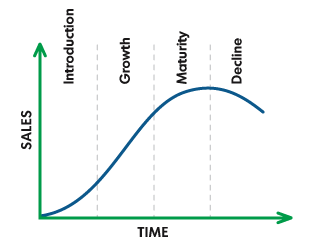
\includegraphics[]{img/product-lifecycle-simple}}\hypertarget{idp54862560}{}%
            \label{idp54862560}
        }
        {{\caption[{Životní cyklus produktu}]{{{Životní 
        cyklus produktu (bez fáze vývoje) \cite{product-lifecycle-graph}}}}\label{fig-product-lifecycle}}}
    \end{center}
\end{figure}

Při vývoji softwaru komerčního licenčního 
typu\footnote{
    Tento typ software je ze zjevných důvodů často nazýván pojmem \glqq 
krabicový software\textquotedblleft{}.}
může být v~principu 
zachován stejný model, liší se pouze délka a množství finančních 
prostředků spotřebovaných v~jednotlivých fázích. Naopak při vývoji 
webové aplikace se životní cyklus poněkud mění. Jak z~pohledu uživatele, 
tak z~pohledu výrobce (tedy například vydavatelské společnosti), se 
smazává rozdíl mezi jednotlivými modely (verzemi) produktu. Webová 
aplikace je obvykle přístupná uživatelům a průběžně se mění, 
zpravidla tak, že většinu inovací uživatel ani nepostřehne. Po úvodní 
fázi vývoje a zavedení produktu se můžou libovolně kombinovat fáze 
růstu, zralosti a útlumu. Lépe řečeno dochází k~opakování životního 
cyklu a ve skutečnosti je vyvíjena nová verze produktu podobným způsobem, 
jako tomu je u~klasických produktů. Vzhledem k~tomu, že rozdíly mezi 
verzemi mohou být velmi 
malé,\footnote{
    Často může jít o~bezpečnostní záplaty nebo drobné optimalizační 
úpravy.
} frekvence iterací 
vývoje a zveřejnění následující verze může být i několikrát denně 
a nová verze po nasazení okamžitě střídá předchozí model webové 
aplikace, tak lze těžko mluvit o~samostatných produktech. Celkově tak 
nastává situace, kdy produkt (resp. služba) funguje nepřetržitě několik 
let, během kterých se ovšem velmi malými obměnami zcela změní. V~duchu 
paradoxu Théseovy lodi přestává být zřejmé, ve kterém momentě a 
případně zda vůbec lze hovořit o~nové verzi produktu. 
\cite{theseus-paradox}{}

V~této souvislosti je obvykle u~klasických produktů používána nová fáze 
životního cyklu, nazvaná rozšíření produktu (\glqq product 
extension\textquotedblleft{}). Pokud výrobce zjistí, že produkt jako takový 
dosahuje poslední fáze životního cyklu, přidáním nových vlastností a 
vylepšení může znovu zvýšit objem prodejů a fázi útlumu oddálit. Jak 
už ale bylo zmíněno v~předchozím odstavci, u~software webového typu nelze 
mluvit přímo o~rozšíření, jako spíše o~nahrazení novým produktem, 
který je ovšem velmi podobný. Graf životního cyklu se tedy mění 
v~spíše tomto duchu, jak ukazuje obrázek 
\hyperlink{fig-product-lifecycle-sw}{{\ref{fig-product-lifecycle-sw}}}.\footnote{
    Ve skutečnosti se nejedná u~každé iterace o~kompletní křivku, ale 
spíše o~navázání na předchozí. Stejně jako rozlišení jednotlivých 
verzí produktu přestává být zřetelné i dělení na původních pět 
Kotlerových fází.}

% figure ------------------------------------------------------
\begin{figure}[hbt]
    \hypertarget{fig-product-lifecycle-sw}{}%
    \begin{center}

        
{{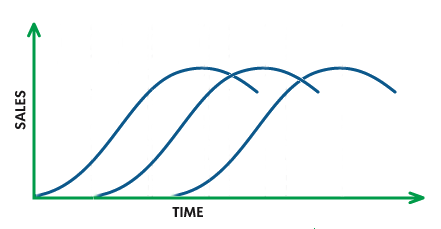
\includegraphics[]{img/product-lifecycle-sw}}\hypertarget{idp54873952}{}%
            \label{idp54873952}
        }
        {{\caption[{Životní cyklus iterativního vývoje webové 
aplikace}]{{{Životní cyklus iterativního vývoje webové 
aplikace}}}\label{fig-product-lifecycle-sw}}}
    \end{center}
\end{figure}

Výše popsané modely životního cyklu softwarového produktu kopírují i 
metodiky vývoje, nasazení a údržby. Konkrétně můžeme zmínit vývoj 
způsobem vodopádu, který je v~současné době u~typických webových 
aplikací považován za překonaný. \cite{waterfall}{} Produkt vyvíjený 
vodopádem kopíruje klasickou křivku životního cyklu. Alternativou je 
iterativní nebo inkrementální způsob vývoje, který vede k~neustálému 
zlepšování existujícího produktu a postupnému přidávání další 
funkcionality (případně odebírání existujících vlastností).
\subsection{Technická omezení}
\label{idp54877232}\hypertarget{idp54877232}{}%

Při návrhu a implementaci inovací softwarového produktu je také potřeba 
brát v~úvahu technická omezení. První skupinou jsou uživatelské 
požadavky, převedené do formy návrhové a implementační specifikace, 
které je prakticky nemožné splnit. Poněkud absurdním příkladem může 
být požadavek na aktualizaci dat ve webové aplikaci i v~případě, že 
zařízení (počítač, chytrý telefon) není připojeno k~internetu. 
Technická omezení splnění takových požadavků jednoduše neumožňují a 
v~rámci vývoje produktu tyto omezení nelze překonat.

Druhým typem omezení jsou taková, která sice překonat lze, nicméně 
stále je potřeba vyvinout netriviální množství úsilí k~dosažení 
takového cíle. Příkladem může být stoprocentní přesnost a aktuálnost 
zobrazovaných dat. Teoreticky sice lze za všech okolností uživateli 
zobrazit naprosto přesná data, například aktuální ceny u~odkazů na 
produkty z~affiliate 
programů,\footnote{
    Některé e-shopy, například Amazon, aktualizují ceny i několikrát za 
hodinu, u~řádově milionů produktů. Technicky je velmi obtížné veškerá 
data okamžitě synchronizovat.
} v~praxi je ovšem často
takové omezení za hranicemi možností realizačního týmu. Taková omezení 
je potřeba zahrnout do procesu vyhodnocování priorit při rozhodování 
o~tom, které vlastnosti (tedy uživatelské požadavky) budou vyvinuty a 
které nikoliv. Samozřejmostí je v~takovém případě i finanční a 
časový odhad vývoje těchto kritických bodů.

V~rámci vývoje software jako řešení affiliate marketingové platformy 
vydavatelské společnosti je kromě standardních technických omezení 
potřeba brát v~úvahu i omezení vyplývající z~povahy zpracovávaných 
dat, jež jsou poskytována třetími stranami. Affliate síť typicky 
zveřejní aplikační programové rozhraní (API), ze kterého je možné 
získávat data (nabídky produktů, aktuální ceny). Bohužel neexistuje 
jednotný standard pro specifikaci těchto dat. Každá síť tak má nastaveny 
parametry přístupu jinak -- často zde existuje omezení limitující počet 
dotazů (požadavků), které API dokáže zpracovat, jindy je omezen zase 
počet produktů, které je možno jedním dotazem získat. Vyvíjený software 
by měl být schopen se v~maximální míře na tyto různorodé podmínky 
adaptovat.

% -------------------------------------------------------------
% Chapter Aplikace affiliate marketingu ve společnosti Future 
% ------------------------------------------------------------- MainMatter
\cleardoublepage\chapter{Aplikace affiliate marketingu ve společnosti Future}
\label{chap-aplikace-am}\hypertarget{chap-aplikace-am}{}%

Společnost Future PLC byla založena v~roce 1985. Jako první vydavatelská 
společnost přišla s~originálním nápadem inovace produktu v~podobě 
tištěného časopisu, totiž jeho rozšíření o~datový nosič, který je 
spolu s~časopisem zabalen v~plastové folii. Tato inovace představovala pro 
zákazníky takovou přidanou hodnotu, že byli ochotni za časopis se 
softwarem zaplatit dvojnásobnou cenu. \cite{independent-chris-anderson}{}

V~praktické části této práce je popsán současný stav provádění 
affiliate marketingu ve společnosti Future, konkrétně v~rámci e-magazínu 
TechRadar. Následně jsou formulovány výzkumné otázky a prostřednictvím 
dotazníku je zjišťováno, v~jakých oblastech lze provádění affiliate 
marketingu zlepšit. Na základě výsledků jsou tato doporučení 
formulována, s~ohledem na zákonitosti affiliate marketingu a technická 
omezení popsaná v~kapitolách \hyperlink{chap-am}{{\ref{chap-am}}} a 
\hyperlink{chap-ecom-soft}{{\ref{chap-ecom-soft}}}. K~vyhodnocení 
dat byly použity programy Google Documents, LibreOffice, Gretl a PSPP.

% ------------------------   
% Section 
\section{Webové magazíny a aplikace pro tablety}
\label{idp54751168}\hypertarget{idp54751168}{}%

Future je stále vydavatelskou společností v~klasickém slova smyslu, 
zabývá se tedy vytvářením a prodejem tištěných magazínů. Stále 
větší váhu nicméně získává elektronická část podnikání. 
\cite{guardian-job-cut}{} Tu tvoří dva hlavní pilíře: webové magazíny a 
aplikace pro tablety.

Pod pojmem webový magazín si můžeme představit soubor webových stránek, 
které obsahují množství tematicky zaměřených článků. Největším 
magazínem tohoto druhu ve společnosti Future je 
TechRadar,\footnote{
    {\textless}\url{www.techradar.com}{\textgreater}
} s~průměrnou
návštěvností přesahující 20 milionů uživatelů měsíčně. 
\cite{youtube-mark-wood-interview}{} Takové velké webové portály jsou 
ideálním místem pro zobrazování affiliate odkazů a sekundárně díky nim 
vhodným způsobem, jak nenásilně velkou návštěvnost monetizovat.

Tato práce se zabývá primárně magazínem TechRadar, a to 
z~následujících důvodů. TechRadar je největším webovým magazínem 
společnosti Future. Zároveň je nejnavštěvovanějším webem o~elektronice 
v~UK a mezi třemi nejčtenějšími magazíny tohoto typu v~USA. TechRadar 
obsahuje články o~elektronice a elektronika je vhodným předmětem affiliate 
marketingu -- lidé ji často nakupují online a rozhodují se na základě 
recenzí a porovnání produktů, jak na základě ceny, tak z~hlediska 
technických parametrů.

Kromě webových e-magazínů ve Future vzniká i několik desítek magazínů 
v~podobě aplikací pro tablety. Technologicky jde jistě o~zajímavé 
produkty, nicméně pro aplikaci affiliate marketingu nejsou vhodnou 
platformou. Problémem je, že v~rámci samostatné aplikace na tabletu 
s~operačním systémem Android nebo iOS uživatel neočekává 
přesměrování do e-shopu. V~mnoha případech by navíc takové řešení 
nebylo ani dost dobře technicky proveditelné, jelikož se aplikace, narozdíl 
od webového magazínu, sama v~prostředí prohlížeče nenachází, a nemusí 
mít od operačního systému oprávnění jinou aplikaci (prohlížeč) 
spustit. Z~těchto důvodů se tímto typem magazínů práce dále do hloubky 
nezabývá a pod pojmem e-magazín je myšlen vždy webový magazín jako 
soubor webových stránek s~tematicky zaměřeným obsahem, pravidelně 
publikovaný na určité doméně.

% ------------------------   
% Section 
\section{Současný stav provádění affiliate marketingu}
\label{chap-soucasny-stav}\hypertarget{chap-soucasny-stav}{}%

V~následující části práce je zhodnocen způsob, kterým společnost 
pracuje s~nástroji affiliate marketingu. Stav, který je v~této kapitole 
popisován jako \glqq současný\textquotedblleft{}, odpovídá situaci 
přibližně z~února 2014. Tedy době, ve které byla data pro analytickou 
část práce sbírána a vyhodnocována.

Společnost Future figuruje v~modelu affiliate marketingu jako vydavatel. 
V~rámci e-magazínu TechRadar vydává řádově jednotky nových článků 
zpravodajského typu, informující o~novinkách ve světě technologií. Mimo 
to publikuje denně přibližně jednu až pět recenzí, v~nichž autor 
hodnotí vlasnosti vybraného produktu -- typicky spotřební elektroniky. 
Recenze obsahuje několik fotek, popis vlastností produktu, provnání 
s~alternativami (jak staršími modely od téhož výrobce, tak srovnání 
s~konkurencí) a odkazy do e-shopů, kde si může čtenář produkt zakoupit. 
Právě poslední zmíněná část úzce souvisí s~affiliate marketingem.
\subsection{Cenové srovnání}
\label{idp54919648}\hypertarget{idp54919648}{}%

Většina recenzí je specificky zaměřena na jeden produkt -- konkrétní 
model, který je recenzí zhodnocen. Ačkoli je u~recenze zobrazeno více 
odkazů, všechny vedou na nákup tohoto stejného modelu produktu. Liší se 
pouze e-shop, do kterého odkaz vede, a samozřejmě parametry specifické pro 
konkrétní nabídku produktu -- zejména cena, dodací lhůta a poplatek za 
doručení zboží.

Tento přístup lze hodnotit ambivalentně. Pozitivní je jednoduchost, kterou 
takový seznam nabízí. Jedná se o~cenové srovnání různých nabídek 
téhož produktu. Lze tedy jasně srovnat, která nabídka je výhodnější. 
Zejména v~oblasti spotřební elektroniky, kde všechny výrobky téhož typu 
pocházejí od jednoho výrobce a liší se pouze distributoři -- tedy různé 
e-shopy. Kromě ceny tak lze porovnávat doručovací lhůtu a cenu doručení, 
celkovou dostupnost produktu a poněkud méně exaktně i dobré jméno e-shopu.

Jak je uvedeno v~kapitole 
\hyperlink{chap-role-am-v-nakupnim-procesu}{{\ref{chap-role-am-v-nakupnim-procesu}}}, 
pro vydavatelskou společnost je zásadní, aby zákazník učinil \glqq 
poslední krok\textquotedblleft{} do e-shopu právě z~daného e-magazínu. Je 
potřeba čtenáře (a tedy potenciálního zákazníka) přesvědčit o~tom, 
že zobrazené porovnání cen je vyčerpávající. Pokud má uživatel pocit, 
že porovnání není kompletní, je pro něj v~prostředí webu velmi 
jednoduché si jít ověřit cenu jinam. Poslední krok do e-shopu je pak 
proveden z~odlišného webu a ačkoliv většinu informací získal čtenář 
z~recenze e-magazínu, affiliate provize putuje jinam.

Zmíněná úplnost se týká zejména počtu e-shopů, které jsou 
v~porovnání zahrnuty. Často se ovšem stává, že i v~rámci jednoho 
e-shopu existuje několik různých nabídek téhož produktu -- například 
portál eBay, na kterém jsou často k~dispozici použité výrobky prodávané 
v~podstatě systémem dražby. V~takovém případě nestačí uvést jednu 
reprezentativní nabídku, ale je potřeba zahrnout různé varianty. Pro 
zmíněný obchod eBay toto v~současném systému porovnání cen funguje, 
nicméně například v~případě Amazonu nejsou zahrnuty nabídky z~Amazon 
Marketplace, což lze vnímat jako potenciální nedostatek.
\subsection{Zobrazení nabídek}
\label{idp54926368}\hypertarget{idp54926368}{}%

Cenové srovnání je u~každé recenze umístěno v~pravé části stránky, a 
rovněž pod recenzí. V~těchto oblastech je ovšem rozložení celé stránky 
nedovoluje uvést kompletní seznam, takže blok obsahuje jen 4 vybrané 
nabídky, označené jako \glqq best deals\textquotedblleft{}. Čtenáři 
ovšem nemusí být jasné, podle jaké logiky jsou tyto nabídky vybrány. Ve 
skutečnosti za jejich výběrem stojí poměrně sofistikovaný algoritmus, 
kombinující cenu, doručovací podmínky, přítomnost slevových kuponů a 
další faktory. Náhled úvodní stránky recenze s~postranním panelem je 
zobrazen v~příloze jako obrázek \hyperlink{fig-widget}{{\ref{fig-widget}}}.

Stejný algoritmus pak stojí za řazením produktů v~úplném cenovém 
srovnání, na které je uživatel přesměrován po kliknutí na odkaz \glqq 
Where to buy\textquotedblleft{} v~menu recenze, nebo \glqq View all 
deals\textquotedblleft{} v~postranním panelu. V~tabulce zahrnující všechny 
dostupné nabídky sice už uživatel má možnost zvolit vlastní řazení, 
nicméně implicitní pořadí nabídek je opět skryto a na první pohled 
postrádá jakoukoli logiku. Jak ukazuje obrázek 
\hyperlink{fig-price-comparison}{{\ref{fig-price-comparison}}} v~příloze 
práce, celkové cenové srovnání má formu tabulky obsahující logo 
e-shopu, název produktu, cenu (s~dodatkem \glqq od\textquotedblleft{}, kterou 
se vydavatel do jisté míry zbavuje odpovědnosti za nepřesnosti), cenu 
poštovného a dodací lhůtu. V~posledním sloupci je pak explicitní odkaz 
\glqq Buy now\textquotedblleft{}, po jehož kliknutí je zákazník 
přesměrován do e-shopu. Je otázkou, zda má smysl uvádět například 
název produktu, vzhledem k~tomu, že cenové srovnání zahrnuje různé 
nabídky, vždy ovšem jednoho stejného produktu, jež je předmětem recenze.

Kromě implicitního řazení, o~kterém již byla řeč, má uživatel 
možnost tabulku cenového srovnání seřadit podle libovolného sloupce, 
včetně jména e-shopu a názvu produktu. Zejména řazení podle názvu 
produktu může být v~mnoha případech zbytečné a pro uživatele matoucí. 
Z~pohledu vývojáře aplikace je logické nabídnout řazení podle všech 
dostupných atributů, nicméně pro uživatele to nemusí znamenat přidanou 
hodnotu. Naopak řazení podle ceny nemusí být na první pohled uživateli 
úplně zřejmé. Různými přístupy k~řazení výsledků, které je často 
klíčové pro správnou interpretaci zobrazovaných dat, se dále zabývá 
výzkum v~kapitole \hyperlink{chap-vyzkum}{{\ref{chap-vyzkum}}}.
\subsection{Slevové kupony}
\label{idp54936688}\hypertarget{idp54936688}{}%

Kromě nabídek samotných produktů je v~tabulce cenového srovnání (jak 
v~náhledu u~recenze, tak v~úplné verzi) sloupec \glqq 
Offers\textquotedblleft{}, obsahující informaci, zda jsou k~nabídce daného 
e-shopu k~dispozici slevové kupony neboli vouchery. Jak už název napovídá, 
tyto slouží jako speciální nabídky e-shopu, obvykle časově omezené. 
Mohou mít formu slevy na konkrétní produkt, určitý typ nebo kategorii 
výrobků, nabídky doručení zdarma nebo výhodné koupě při kombinaci 
určitého zboží (například tašku na notebook zdarma při koupi 
přenosného počítače).

V~současné podobě zobrazované v~e-magazínu slevové kupony často 
neodpovídají produktu, ke kterému jsou přiřazeny. Například u~herní 
konzole XBox můžeme najít poukázku na 10\% slevu při nákupu ledničky. 
Pro uživatele pak může být takový slevový kupon matoucí. Navíc se 
často stává, že je k~nabídce přiřazeno několik desítek voucherů, 
z~nichž je ale jen několik málo skutečně relevantních. Bohužel ani 
v~tomto případě není možno irelevantní vouchery jednoduše vyfiltrovat.

Z~technického pohledu je výše popsaný nedostatek způsoben faktem, že 
slevové kupony jsou automaticky zpracovávány systémem, který nedisponuje 
sémantickou analýzou textu a není tedy možné pomocí něj zjistit, zda je 
voucher pro konkrétní produkt relevantní. V~rámci výzkumu je proto 
testováno, do jaké míry jsou slevové kupony pro zákazníky důležité, a 
zda má větší smysl investovat zvýšení jejich relevance, nebo na druhou 
stranu jejich úplné vyřazení ze systému.
\subsection{Uživatelské komentáře}
\label{sect-user-reviews-current}\hypertarget{sect-user-reviews-current}{}%

Čtenářské diskuse jsou v~dnešní době standardní součástí 
e-magazníů. Obzvláště u~recenzí, kde se ke konkrétnímu výrobku 
z~kategorie spotřební elektroniky vyjadřuje editor, čtenáři e-magazínu 
často chtějí znát i názor dalších (běžných) spotřebitelů a jejich 
zkušenosti s~popisovaným výrobkem. Hodnocení ostatních čtenářů se tak 
vlastně stává součástí recenze.

Současná podoba e-magazínu TechRadar zobrazuje komentáře ostatních 
uživatelů všem návštěvníkům webu, ale přispívat mohou pouze 
registrovaní uživatelé. Tím je na jedné straně zajištěna určitá 
úroveň příspěvků a nemožnost diskusi zahltit spamem, na straně druhé 
určitá překážka pro čtenáře, který chce do diskuse přispět, ovšem 
nemá vytvořený uživatelský účet.

Komentáře samotné jsou řazeny stylem top-post, tedy nejnovější 
komentář je nahoře. Podobně jsou uveřejňovány novinky na sociálních 
sítích Facebook a Twitter nebo komentáře na video-serveru YouTube. Naopak 
většina zpravodajských médií řadí komentáře uživatelů chronologicky, 
tedy nový příspěvek je zobrazen v~diskusi jako poslední. Obzvláště 
v~případě, kdy na sebe komentáře reagují nebo se jedná o~delší texty, 
je čtení top-post příspěvků náročnější. \cite{top-posting}{}

V~současné podobě jsou komentáře moderovány editory e-magazínu. Pokud se 
tedy v~diskusi objeví vulgární nebo nevhodný příspěvek, může být 
smazán. Sami uživatelé ovšem nemají možnost sekundární zpětné vazby, 
tedy hodnocení komentářů ostatních čtenářů. Neexistuje prosté 
hlasování pro kvalitní komentář, není zde možnost nahlásit nevhodný 
komentář ani na konkrétní příspěvek přímo reagovat.

I~uživatelské komentáře a zapojení čtenářů při nákupu jsou 
součástí marketingového výzkumu.
\subsection{Konkurence}
\label{idp54947424}\hypertarget{idp54947424}{}%

Při hodnocení jakéhokoli produktu nebo služby bývá důležité srovnání 
s~konkurencí. Nejinak je tomu i v~případě provádění affiliate marketingu 
vydavatelskou společností Future. Podobných produktů, nabízejících 
čtenáři hodnocení v~podobě recenze, cenové srovnání a další 
související informace, je totiž na internetu celá řada. V~této sekci jsou 
diskutovány shody a odlišnosti oproti tomu, co čtenáři vidí 
v~součansnosti v~rámci e-magazínu TechRadar.

Na prvním místě pro srovnání je americký e-magazín 
cNet,\footnote{
    {\textless}\url{http://cnet.com}{\textgreater}
} zaměřený podobně jako
TechRadar na novinky a recenze z~oblasti spotřební elektroniky. Struktura 
recenze je velmi podobná TechRadaru. Text a obrázky recenze jsou na pravé 
straně doplněny vybranými nabídkami produktu. Pod samotnou recenzí je 
stejně jako v~případě TechRadaru diskuse a hodnocení samotných 
uživatelů. Struktura diskuse se ovšem poněkud liší. Komentáře na sebe 
totiž mohou navazovat a vytvářet skutečnou diskusi.

Cenové srovnání všech nabídek na cNetu je velice podobné TechRadaru. 
S~pomocí některého z~nástrojů na prohlížení historie 
webu\footnote{
    Například {\textless}\url{http://archive.org/web/}{\textgreater}
} lze vidět, že oba
e-magazíny provedly vizuální inovaci na podzim roku 2013.

Prvním viditelným rozdílem cNetu oproti TechRadaru je absence slevových 
kuponů. Pokud je nabídka něčím speciální, je tato informace uvedena 
v~čistě textové podobě jako doprovodný popisek. Zajímavým a na první 
pohled kosmetickým rozdílem je popisek tlačítka, kterým uživatel přejde 
z~e-magazínu do e-shopu. V~případě cNetu tento popisek nese název \glqq 
See it\textquotedblleft{}, zatímco TechRadar uživateli předkládá \glqq Buy 
now\textquotedblleft{}. Zejména u~méně zkušených uživatelů může 
popisek \glqq Buy now\textquotedblleft{}, tedy doslova \glqq Koupit 
teď\textquotedblleft{}, vzbuzovat určité obavy z~toho, že kliknutím na 
odkaz už provádí nákup, zatímco ve skutečnosti si chtějí jen nabídku 
prohlédnout, přesně jak jim tlačítko prezentuje cNet. Reálně lze tento 
rozdíl změřit A/B testováním. \cite{ab-testing}{} V~duchu zadání této 
práce uživatelské testování software prováděno nebylo, jedná se však 
o~možnost dalšího rozpracování tématu a navázání na základní 
poznatky zde uváděné.

Kromě zmíněného cenového srovnání nabízí cNet dvě řešení, která 
na TechRadaru zcela chybí. Prvním z~nich je cenové srovnání podobných 
produktů. Pokud si tedy čtenář e-magazínu přečte recenzi například 
o~telefonu Samsung Galaxy S5, je mu nabídnuto srovnání parametrů a 
cenových nabídek se starším modelem S4 nebo konkurenčním iPhone 6. 
V~rámci dotazníkového šetření, popsaného v~kapitole 
\hyperlink{chap-vyzkum}{{\ref{chap-vyzkum}}}, je zjišťováno, jak čtenáři 
takové srovnání vnímají a zda má smysl ho zařadit do magazínu TechRadar.

Druhým prvkem, kterým cNet předstihuje TechRadar v~bohatosti funkcionality, 
je analýza cenového trendu. Uživatel má možnost zobrazit si v~grafu 
historii cen a dokonce si nastavit upozornění, které mu zašle e-mail 
v~případě, že cena klesne pod určitou hranici. Tato funkcionalita má 
smysl v~případě, že cena je pro zákazníka rozhodujícím parametrem. 
Naopak proti zavedení takové funkcionality by hovořil fakt, že zákazník, 
který se rozhodne koupit si daný produkt, s~nákupem obvykle nechce 
vyčkávat. Oba faktory jsou také zahrnuty do marketingového výzkumu.

Dalším z~poskytovatelů služby z~oblasti affiliate marketingu je Google, 
v~rámci platformy Google Shopping. Uživateli je nabídnuto cenové srovnání 
podobné tomu na TechRadaru nebo cNetu. Nejzajímavějším rozdílem je 
sloučení ceny produktu s~poštovným. Zákazníkovi je tak tedy přehledně 
zobrazena celková cena, kterou za náku produktu zaplatí. Na druhou stranu 
takové srovnání nebere v~úvahu možnost vyzvednutí zboží na prodejně, 
která je zejména u~méně zkušených zákazníků nebo menších e-shopů 
často preferována. Google také kromě řazení produktů nabízí 
jednoduché filtrování, kterým je možné vybrat například pouze nabídky, 
u~nichž je poštovné zdarma.

Zajímavým portálem pracujícím jako affiliate partner je česká Heuréka. 
Tento portál se zaměřuje na srovnání nabídek produktů, podobně jako 
TechRadar nebo cNet. Neomezuje se ale jen na přesměrování zákazníků do 
různých e-shopů, ale zboží je možno nakoupit přímo na tomto portálu. 
Nejedná se o~internetový obchod v~klasickém slova smyslu, který by 
zajišťoval i skladování a předání fyzického zboží, protože i 
objednávka dokončená na portálu Heuréka je realizována v~některém 
z~konkrétních partnerských e-shopů. Z~pohledu uživatele může ale toto 
odstínění znamenat několik výhod. První z~nich je fakt, že pokud je 
nákup prováděn častěji, pokaždé se zákazník pohybuje ve stejném 
uživatelském rozhraní, nehledě na to, který e-shop zrovna disponuje 
nejlepší nabídkou. Druhou výhodou je určitá úroveň garance, kterou 
může Heuréka nabídnout při nákupu z~méně známých e-shopů.

Posledním významným rozdílem, který byl identifikován na portálu 
Heuréka, ale vyskytuje se i u~jiných affiliate služeb, je rozšíření 
nabídky o~příslušenství k~produktu. Pokud má zákazník zájem o~telefon 
iPhone 5, kromě cenového srovnání a nabídek tohoto přístroje jsou mu 
zobrazeny možnosti koupě napájecího kabelu, ochranného obalu nebo 
hands-free sady. U~tohoto přístupu je pozitivem potenciální rozšíření 
počtu zákazníků. Nabídka může zaujmout i někoho, kdo už iPhone 5 
vlastní. Na druhou stranu v~rámci e-magazínu obsahujícího recenze 
produktů lze předpokládat, že valnou většinu čtenářů budou tvořit 
právě zákazníci, které zajímá především produkt samotný. 
I~z~finančního hlediska je pro affiliate program e-magazínu mnohem 
výhodnější zprostředkovat nákup drahého telefonu, než řádově 
levnějšího příslušenství. Procentuálně konstantní provize je totiž 
v~prvním případě, přepočítána na konkrétní částku, také řádově 
vyšší.

% ------------------------   
% Section 
\section{Marketingový výzkum}
\label{chap-vyzkum}\hypertarget{chap-vyzkum}{}%

Na základě uvedeného popisu současného stavu provádění affiliate 
marketingu, a to jak přímo v~rámci e-magazínu TechRadar, tak na 
konkurenčních portálech, je vidět, že zde existuje prostor pro inovaci. 
Vylepšování a obměňování softwarového produktu ale nelze provést pouze 
na základě úsudku. Inovace musí být založeny na objektivních datech 
reflektujících názor a očekávání uživatelů portálu. Jednou z~metod 
získání takových dat je marketingový výzkum formou dotazníku, který byl 
v~rámci této práce proveden a je popsán a zhodnocen v~této kapitole. 
Dalšími možnostmi pro získání informací, které však v~rámci této 
práce nebyly využity, by mohl být rozhovor s~několika stávajícími 
uživateli, uživatelské testování nebo A/B testování.

Jedním z~důvodů, proč nebyla využita statistická data dokumentující 
provoz (pohyb uživatelů v~rámci e-magazínu), je silné zkreslení takových 
informací. Vzhledem k~velmi snadné dostupnosti konkurenčních produktů 
uživatel, pokud není s~kvalitou produktu, resp. poskytované služby v~rámci 
e-magazínu spokojen, stránku rychle opouští. Některé zdroje uvádí, že 
více než polovina uživatelů webovou stránku opustí do 15 sekund. 
\cite{time-15-sec}{} Důvody nespokojenosti takových uživatelů je pak ze 
statistických dat provozu velmi těžké identifikovat. Proto je dotazník 
zaměřen, ve smyslu zadání práce, zejména na očekávání a obecné 
vzorce chování při nakupování na internetu, a tedy potenciálně 
využívání prostředků affiliate marketingu.

\subsection{Metodika výzkumu}
\label{idp54973536}\hypertarget{idp54973536}{}%

Provedený marketingový výzkum má kvantitativní povahu. Obecným 
výzkumným cílem je identifikace míry naplnění požadavků a očekávání 
od v~současnosti nabízeného produktu z~oblasti affiliate marketingu, který 
je popsán v~sekci \hyperlink{chap-soucasny-stav}{{\ref{chap-soucasny-stav}}}. 
Na základě principů fungování affiliate marketingu, popsaných v~kapitole 
\hyperlink{chap-am}{{\ref{chap-am}}}, a teorie nákupního rozhodování, 
kterému se věnuje sekce 
\hyperlink{chap-nakupni-rozhodovani}{{\ref{chap-nakupni-rozhodovani}}}, byly 
formulovány následující obecné výzkumné otázky, zjišťující 
očekávání z~pohledu čtenářů e-magazínu:

\begin{itemize}
        %--- Item
    \item 
        Jaký má být obsah webového produktu vytvořeného na základě 
affiliate marketingu?

        %--- Item
    \item 
        Na základě jakých kritérií by měl být obsah seřazen a 
prioritizován?

        %--- Item
    \item 
        Jak přesné a aktuální informace je potřeba uživatelům poskytnout?

        %--- Item
    \item 
        Jakým způsobem by měli samotní uživatelé spoluvytvářet produkt?\footnote{
            Z pohledu e-commerce platformy je spoluúčast na tvorbě produktu reprezentována typicky 
            uživatelskými komentáři s hodnocením jednotlivých produktů či celých e-shopů.
        }

\end{itemize}
\noindent 
Pro každou z~těchto obecný výzkumných otázek jsou následně formulovány 
konkrétní otázky, z~nichž je sestaven dotazník obsahující 25 otázek. 
Každá z~těchto otázek už je poměrně specifická a váže se na 
konkrétní aspekt očekávání. \cite{navrh-vyzkumu}{} Kompletní dotazník 
je součástí \hyperlink{appendix-dotaznik}{přílohy}.

Tato práce zjišťuje požadavky a 
očekávání\footnote{
    U~produktu zkoumaného typu se požadavky a očekávání překrývají. 
Lze konstatovat, že pokud čtenář e-magazínu očekává funkcionalitu~X, je 
jeho uživatelským požadavkem získat funkcionalitu~X.
} potenciálních
uživatelů produktu z~oblasti affiliate marketingu, tedy čtenářů 
e-magazínu. Primárně se tedy nezabývá vzájemným vztahem zkoumaných 
veličin, nýbrž jejich absolutní hodnotou. Proto jsou všechny otázky 
uzavřené a pro odpovědi byla zvolena pětibodová škála. Lichý počet 
variant zajišťuje, že odpovídající není nucen vždy vybírat pozitivní 
nebo nebo negativní odpověď, potenciálně tedy získaný vzorek dat lépe 
odpovídá realitě. Vzhledem k~povaze otázek, které často přímo 
zjišťují subjektivní míru očekávání nebo názor respondenta, by více 
než pět bodů na škále nepřineslo větší přesnost odpovědí. Naopak by 
mohlo docházet k~nežádoucímu jevu, kdy dva respondenti s~podobně 
vyhraněným názorem vyberou na škále dvě podobné, nikoli však stejné, 
odpovědi. Pětibodová stupnice se tak jeví jako ideální.

Dotazník je sestaven tak, aby na základě odpovědí bylo možno rozhodnout, 
které vlastnosti produktu uživatelé očekávají, případně co konkrétně 
by tyto vlastnosti měly obsahovat a jakým způsobem by měly být 
zobrazovány. Na základě těchto vlastností jsou v~této kapitole jednak 
ověřeny stávající vlastnosti produktu, dále jsou pak navrženy možné 
způsoby inovace.

Dotazovanou cílovou skupinou jsou muži ve věku mezi 20 a 30 lety, kteří 
tvoří podle tvrzení společnosti Future většinu čtenářů e-magazínu. 
Rozhodl jsem se ale do průzkumu zahrnout i ženy, protože srovnání 
nákupního chování žen a mužů by mohlo odhalit zajímavé body, na které 
se lze při inovaci zaměřit, přizpůsobit produkt i ženské části 
populace a potenciálně tak počet čtenářek zvýšit. Aby byl ovšem 
průzkum validní v~rámci zadání, je základní analýza provedena na vzorku 
obsahujícím odpovědi mužských respondentů. Až následné rozšíření 
řeší rozdíly mezi muži a ženami v~rámci celého vzorku dotazovaných.
\subsection{Dotazník}
\label{idp54989728}\hypertarget{idp54989728}{}%

Pro obecné výzkumné otázky uvedené v~předchozí kapitole byly 
identifikovány konkrétní otázky obsažené v~dotazníku. Prvních 6 otázek 
zjišťuje charakteristiky respondenta samotného; tedy pohlaví, věk, 
vzdělání, frekvenci nákupu v~e-shopech a odhad částky, která je takto 
utracena. Důvodem pro zařazení těchto otázek je validace cílové skupiny 
-- tedy zjištění, zda a případně jakým způsobem jsou odpovědi 
specifické pro mužskou část respondentů, která byla identifikována jako 
majoritní segment. Díky zahrnutí těchto otázek tak lze jednoduše zkoumat 
nejen odlišnosti mezi muži a ženami, ale závislost odpovědí na dalších 
parametrech, jako je frekvence nákupů či průměrná částka utracená 
v~e-shopech s~elektronikou. Poslední zmíněná metrika může být pro 
vydavatele velmi zajímavá, protože provize je počítána jako 
procentuální díl právě z~ceny prodaného zboží.

Následujících 6 otázek, tedy čísla 7 až 12, se vztahuje k~první obecné 
výzkumné otázce. Řeší tedy, jaké aspekty jsou obsahově pro uživatele 
důležité. Tyto otázky byly formulovány na základě současného stavu 
produktu a analýzy podobných konkurenčních produktů.

Další výzkumné otázce, tedy problematice řazení a prioritizace obsahu, 
je věnováno 7 otázek s~pořadovými čísly 13 až 19. Problémem, který si 
tato část klade za úkol vyřešit, je fakt, že uživateli není možno 
zobrazit vyčerpávající seznam všech nabídek produktů, obzvláště 
v~případě, kdy by seznam měl obsahovat nejen jeden konkrétní model, ale i 
podobné produkty od dalších výrobců. Rozumnějším přístupem se jeví 
jistá míra předfiltrování zobrazovaných dat. Poskytovatel služby, tedy 
vydavatelská společnost, na základě výzkumu může identifikovat 
nejdůležitější parametry, podle kterých vybere \glqq 
nejlepší\textquotedblleft{} nabídky. Právě odpověď na otázku, co 
znamená nejlepší, má zodpovědět tato část.

I~v~případě, by uživatelé preferovali vlastní výběr z~delšího 
seznamu,\footnote{
    Jak je vidět dále v~analýze odpovědí, uživatelé skutečně 
preferují výběr z~více než několika jednotek nabídek, které za ně 
vybere vydavatel.
} je zapotřebí tento
seznam nějakým způsobem seřadit a nabídnout v~rámci služby možnosti 
filtrování a řazení. Bez nich prakticky není možno rozumně pracovat 
s~více než několika málo desítkami záznamů.

Otázka 20 zkoumá, zda má smysl se v~rámci vývoje orientovat na mobilní 
platformy. V~dnešní době je standardem při tvorbě webové aplikace 
vytvořit i verzi přizpůsobenou prohlížení na telefonu. Tato otázka ale 
řeší, jestli je mobilní telefon skutečně plnohodnotným zařízením, ze 
kterého uživatel provede i nákup v~e-shopu, nebo slouží jen jako čtečka 
e-magazínu. V~druhém případě totiž mobilní uživatelé nepřináší 
vydavatelské společnosti z~affiliate programu žádný příjem.

Otázka s~číslem 21 spadá tematicky pod řazení obsahu, nicméně ptá se 
konkrétně na označení tlačítka, kterým je možno obsah uspořádat. 
Jinými slovy zkoumá, jaký text na tomto tlačítku je pro uživatele 
nejpochopitelnější. Zajímavostí je, že při konzultaci dotazníku 
s~vydavatelskou společností (ještě před sesbíráním a vyhodnocením 
odpovědí) bylo původní tlačítko \glqq vzestupně\textquotedblleft{} 
vyměněno za \glqq od nejnižšího k~vyššímu\textquotedblleft{}. Takže 
první reálná inovace byla provedena na základě této práce ještě 
dříve, než byly publikovány jakékoli výsledky výzkumu.

K~otázce 22 je potřeba říct, že v~současné době nejsou v~cenovém 
srovnání na TechRadaru uváděny produkty, které jsou momentálně v~daném 
e-shopu nedostupné. Z~hlediska politiky maximalizace konverze a počtu 
uskutečněných nákupů to dává smysl, nicméně z~pohledu uživatele to 
tak nutně být nemusí. Proto jsem vytvořil hypotézu, že zákazník 
v~případě pořízení elektroniky raději nákup o~několik dní odloží, 
pokud jde o~výhodnou, ale momentálně nedostupnou nabídku. Právě 
zmíněná hypotéza je testována tímto bodem. Otázka 23 zjišťuje, zda má 
smysl affiliate odkazy zobrazovat i jako reklamní bannery. Poslední dvě 
otázky řeší, jak důležitá je součást produktu spoluvytvářená 
samotnými čtenáři -- tedy uživatelské komentáře.

Většina otázek byla formulována na základě kombinace analýzy 
stávajícího produktu, jeho historického vývoje, posouzení konkurenčních 
produktů a uvážení mechanismů affiliate marketingu. Zejména u~otázek 22 
a 23 byly při konstrukci otázky využity principy nákupního chování, 
popsané v~kapitole 
\hyperlink{chap-nakupni-rozhodovani}{{\ref{chap-nakupni-rozhodovani}}}.

Vzhledem k~povaze zkoumaného problému, kterým je webová aplikace z~oblasti 
affiliate marketingu, byl dotazník distribuován také elektronicky, a to 
prostřednictvím sociálních sítí. Ačkoliv vydavatelská společnost 
Future působí ve Velké Británii a produkt je vytvářen v~angličtině, 
tato práce je psána česky a vzorek dotazovaných byl složen z~českých 
respondentů. Tento fakt může způsobit drobné zkreslení dat, nicméně 
vzhledem ke globální povaze affiliate marketingu a celkové podobnosti 
těchto platforem (např. již zmíněná česká Heuréka) pravděpodobně 
nepůjde o~významnější problém, který by bránil správné interpretaci 
dat.

V~rámci obecných výzkumných otázek byl také nastíněn problém 
aktuálnosti a přesnosti informací. Velké množství dat, se kterými 
affiliate systém musí pracovat, prakticky znemožňuje mít veškeré 
informace vždy přesné a aktuální, tak jak bylo popsáno v~kapitole 
\hyperlink{chap-ans}{{\ref{chap-ans}}}. Do dotazníku nicméně otázky na toto 
téma zařazeny nebyly. Důvodem je fakt, že uživatelé chtějí maximálně 
přesné a aktuální informace, na to není potřeba se jich ptát. V~rámci 
celkové analýzy a doporučených inovací je ale aktuálnost a přesnost 
poskytovaných dat zahrnuta, ačkoliv se nejedná o~metriku, která by mohla 
být zjišťována marketingovým 
dotazníkem.\footnote{
    K~dotazníku byl také připojena informace, slibující jednomu náhodně 
vybranému respondentovi finanční odměnu ve výši 500 Kč. Důvodem této 
pobídky byla snaha získat maximální množství relevantních odpovědí. 
Vzhledem k~tomu, že celkový počet odpovídajících přesahuje 200, lze 
považovat tento bod za funkční.
}
\subsection{Odpovědi respondentů}
\label{idp55010672}\hypertarget{idp55010672}{}%

V~této části práce jsou analyzovány agregované odpovědi respondentů. 
Jak již bylo zmíněno, většina otázek nabízí odpovědi na uzavřené 
pětibodové škále, dále reprezentované číselnými hodnotami 0 až 4. 
Tato uniformita umožňuje vzájemné porovnání číselných reprezentací 
odpovědí jednotlivých otázek, a tedy i porovnání priorit z~pohledu 
uživatele. Odpovědi na každou otázku tedy byly vyhodnocovány jako 
výběrové náhodné veličiny založené na odpovědích 89 mužských 
respondentů.

Tabulka \hyperlink{tobsah}{{\ref{tobsah}}} zobrazuje číselné charakteristiky 
odpovědí na otázky 7 až 12. Ukazuje se, že tři základní pilíře 
affiliate marketingu ve společnosti Future mají smysl: většina uživatelů 
má zájem o~recenze elektroniky, doplněné o~obrázky a fotografie produktů, 
a následně využije služby cenového srovnání. Střední hodnota ve výši 
3,76 a malý rozptyl odpovědí na otázku č. 10 ukazují, že v~očekávání 
uživatelů je porovnání alternativ, tedy podobných produktů v~rámci 
stejné kategorie, ještě o~něco výše než recenze a cenové srovnání 
nabídek jednoho konkrétního produktu.

Základní odpovědí na první výzkumnou otázku, zabývající se 
zobrazovaným obsahem, je tedy to, že stávající podoba obsahující 
recenzi, obrázky produktu a cenové srovnání je v~pořádku. Cenové 
srovnání, a potažmo i recenze samotná, by měly být rozšířeny 
o~srovnání s~podobnými produkty.

% table ------------------------------------------------------
\begin{table}[htb]
    \begin{center}%
       % \hypertarget{tobsah}{\label{tobsah}}
        \begin{tabular}{|c|c|c|}
            \hline 
            {{}} & {{Střední hodnota}} & {{Směrodatná odchylka}} 
\tabularnewline
             \hline 
             {{Recenze produktu}} & {{3.5618}} & {{0.6564}} \tabularnewline
              \hline 
              {{Cenové srovnání}} & {{3.0000}} & {{0.9535}} \tabularnewline
               \hline 
               {{Vyhledávání podle parametrů}} & {{3.7640}} & {{0.4270}} 
\tabularnewline
                \hline 
                {{Zahrnutí podobných produktů}} & {{2.4944}} & {{1.2259}} 
\tabularnewline
                 \hline 
                 {{Obrázky}} & {{3.9213}} & {{0.2707}} \tabularnewline
                  \hline 
                  {{Exkluzivní nabídka (sleva)}} & {{1.3258}} & {{0.7801}} 
\tabularnewline
                  \hline 
              \end{tabular}
              \caption{Obsah produktu -- popisné statistiky}\label{tobsah}
          \end{center}
      \end{table}

      Další výzkumná otázka se zabývá prioritizací obsahu. Jinými 
slovy řeší, které aspekty jsou při online nakupování zákazníky 
vnímány jako nejpodstatnější. V~současné době jsou totiž zobrazované 
nabídky řazeny algoritmem kombinujícím parametry uvedené v~tabulce 
\hyperlink{tab-prioritizace}{\ref{tab-prioritizace}}. Každému parametru je přiřazena určitá 
váha, která určuje celkové pořadí. Vzhledem k~přibližně podobným 
směrodatným odchylkám všech náhodných veličin můžeme říct, že 
optimální poměr pro řadící algoritmus by měl odpovídat váze 
středních hodnot. Tedy při celkovém součtu 14,38 by měla cena v~celkovém 
řazení reprezentovat přibližně 19\% váhu.

      % table ------------------------------------------------------
      \begin{table}[htb]
          \begin{center}%
              \begin{tabular}{|c|c|c|}
                  \hline 
                  {{}} & {{Střední hodnota}} & {{Směrodatná odchylka}} 
\tabularnewline
                   \hline 
                   {{Nízká cena}} & {{2.7303}} & {{1.0086}} \tabularnewline
                    \hline 
                    {{Slevové kupony}} & {{1.3483}} & {{1.0011}} 
\tabularnewline
                     \hline 
                     {{Dodací lhůta}} & {{2.0899}} & {{1.2214}} 
\tabularnewline
                      \hline 
                      {{Poštovné}} & {{2.4045}} & {{1.3031}} \tabularnewline
                       \hline 
                       {{Zkušenosti s~e-shopem}} & {{3.3483}} & {{0.7848}} 
\tabularnewline
                        \hline 
                        {{Certifikát spolehlivosti}} & {{2.4719}} & {{1.0010}} 
\tabularnewline
                        \hline 
                    \end{tabular}
                    \caption{Prioritizace obsahu -- popisné statistiky}\label{tab-prioritizace}
                \end{center}
            \end{table}

            Na hodnotách z~tabulky prioritizace je vidět, že slevové kupony 
nehrají pro zákazníky velkou roli. V~současné podobě je na ně ovšem 
kladen velký důraz a jsou zobrazovány jak v~náhledu cenového srovnání 
u~recenze, tak v~plném cenovém srovnání. Jednou z~možností je nahrazení 
tohoto sloupce informací o~certifikátu spolehlivosti.

            Nejvyšší prioritu kladou respondenti poměrně překvapivě na 
to, zda mají již s~daným e-shopem zkušenosti. Tento atribut je ovšem 
závislý na konkrétním uživateli. V~kapitole 
\hyperlink{chap-doporuceni}{{\ref{chap-doporuceni}}} jsou diskutovnány 
možnosti rozšíření o~tento aspekt.

            Zvláštní pozici v~otázce prioritizace obsahu zaujímá otázka 
14: \glqq Stačí vám vidět 5 nejlepších nabídek produktu, které za vás 
někdo vybral?\textquotedblleft{}. Jak ukazuje rozložení hodnot odpovědí 
v~grafu \hyperlink{fig-top-5}{{\ref{fig-top-5}}}, většina respondentů 
preferuje vlastní výběr z~většího množství produktů. Cenové 
srovnání přímo na stránce s~recenzí, obsahující pouze pět vybraných 
nabídek, by tedy mělo sloužit především jako navigační komponenta, 
která čtenáře zaujme a po kliknutí ho přesměruje na kompletní cenové 
srovnání. Toto doporučení bude platit i v~případě zahrnutí dalších 
rozšíření produktu o~zobrazení omezeného počtu nabídek.

            % figure ------------------------------------------------------
            \begin{figure}[hbt]
                \hypertarget{fig-top-5}{}%
                \begin{center}

                    
{{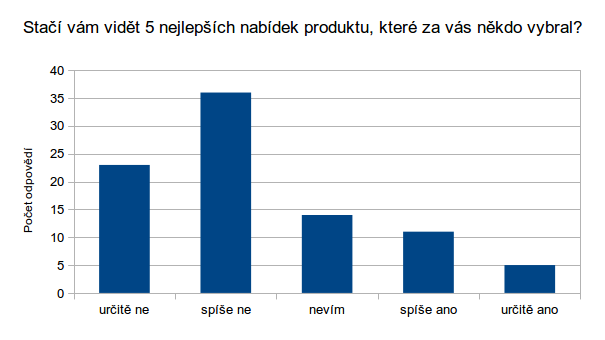
\includegraphics[width=400px]{img/top-5}}\hypertarget{idp55050896}{}%
                        \label{idp55050896}
                    }
                    {{\caption[{Rozložení odpovědí na otázku č. 14 -- 
pouze 5 produktů}]{{{Rozložení odpovědí na otázku č. 14 -- pouze 5 
produktů}}}\label{fig-top-5}}}
                \end{center}
            \end{figure}

            Posledním tématem, kterým se dotazník zabývá, je 
očekávání spoluvytváření produktu pomocí uživatelských komentářů, 
tedy míra jejich důležitosti. Data zobrazená v~grafu 
\hyperlink{fig-user-reviews}{{\ref{fig-user-reviews}}} ukazují, že tato 
součást je pro cílovou skupinu čtenářů e-magazínu typu TechRadar velmi 
důležitá. Žádny z~respondentů neodpověděl zcela negativně, naopak 
naprostá většina takovouto funkcionalitu při online nakupování použije.

            % figure ------------------------------------------------------
            \begin{figure}[hbt]
                \hypertarget{fig-user-reviews}{}%
                \begin{center}

                    
{{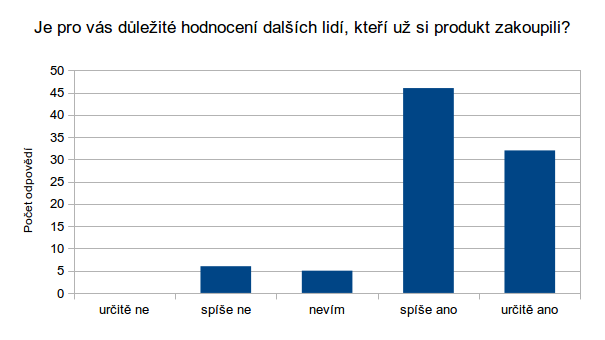
\includegraphics[width=400px]{img/user-reviews}}\hypertarget{idp55055696}{}%
                        \label{idp55055696}
                    }
                    {{\caption[{Odpovědi na otázku č. 24 -- komentáře 
ostatních uživatelů}]{{{Odpovědi na otázku č. 24 -- komentáře 
ostatních uživatelů}}}\label{fig-user-reviews}}}
                \end{center}
            \end{figure}

            \subsection{Vliv různých faktorů na hodnotu nákupu}
            \label{idp55057200}\hypertarget{idp55057200}{}%

            Kromě obecných preferencí a očekávání uživatelů, které 
byly diskutované v~předchozí části, má smysl zodpovědět otázku, zda 
existuje závislost rozložení odpovědí na celkové hodnotě nákupního 
košíku, agregovaného ze všech nákupů (tedy součet hodnot nákupů). 
Nechť dva faktory X a Y mají přibližně stejnou úroveň očekávání 
(například existence recenze a možnost prohlížení si obrázků produktu). 
Pokud X preferují zejména zákazníci, kteří utrácí více, má smysl se 
při inovaci při výběru mezi X a Y zaměřit právě na vývoj X. Naplnění 
takového požadavku totiž vede ke zvýšení spokojenosti právě těch 
zákazníků, kteří na internetu utrácí za elektroniku nejvíce a jsou pro 
vydavatelskou společnost tedy nejcennější.

            K~vyhodnocení otázky z~předchozího odstavce byla použita 
lineární regrese pomocí metody nejmenších čtverců (ordinary least 
squares -- OLS).\index{ordinary least squares} Model byl sestaven nejprve ze 
všech číselných vyjádření otázek 7 až 25. Následně byly z~modelu 
podle pravidel lineární regrese odebírány nevýznamné proměnné. Ukázalo 
se, že proměnné signifikantní na hladině významnosti 10 \% jsou pouze 
tři. Dvě se vztahují ke způsobu doručení zboží (otázky 17 a 18), 
poslední proměnná zachycuje očekávání uživatelů z~pohledu porovnání 
produktu s~alternativami (otázka č. 10). Model je vyjádřen následující rovnicí:

\begin{center}
    %P(x) = \frac{x - a}{b - a} , \nonumber
$ Purchase = 18401.5 - 2237.59*Alt + 4467.33*STime - 4047.22*SCost $
%                    {{\caption{Upravený OLS model vlivu očekávání na agregovanou hodnotu nákupu}\label{eq-ols}}}
\end{center}

Konkrétní hodnoty modelu jsou zobrazeny v~tabulce 
\hyperlink{tab-ols}{\ref{tab-ols}}.
Zde jsou také zahrnuty směrodatné odchylky a p-hodnoty testující relevanci jednotlivých parametrů.

            % table ------------------------------------------------------
            \begin{table}[htb]
                \begin{center}%
                    \begin{tabular}{|c|c|c|c|}
                        \hline 
                        {{}} & {{Koeficient}} & {{Směrodatná chyba}} & {{p-hodnota}} \tabularnewline
                         \hline 
                         {{konstanta}} & {{18401.5}} & {{4587.01}} & {{0.0001}} \tabularnewline
                          \hline 
                          {{Zahrnutí podobných produktů (Alt)}} & {{- 2237.59}} & {{1200.46}} & {{0.0658}} \tabularnewline
                           \hline 
                           {{Dodací lhůta (STime)}} & {{4467.33}} & {{1376.22}} & {{0.0017}} \tabularnewline
                            \hline 
                            {{Poštovné (SCost)}} & {{- 4047.22}} & {{1289.46}} & {{0.0023}} \tabularnewline
                            \hline 
                        \end{tabular}
                        \caption{Koeficienty OLS modelu s~p-hodnotami}\label{tab-ols}
                    \end{center}
                \end{table}

                OLS model není nejpřesnějším vyjádřením závislosti, 
zejména v~případě, kdy všechny vysvětlující proměnné jsou umělé, 
jelikož jejich číselné vyjádření je pouze číselnou reprezentací 
diskrétní pětibodové škály. Konstanta je v~tomto případě zcela 
bezvýznamná, jelikož stupnici škály lze reprezentovat libovolnou linární 
řadou. Nicméně, přibližně je z~OLS modelu vidět, že pro zákazníky, 
kteří v~průměru více utrácejí, je důležitá dodací lhůta. Bez ohledu 
na model je tento fakt vcelku logický, neboť je pravděpodobné, že jde 
o~zkušenější uživatele zaměřující se více na dražší novinky. 
Naopak lidé, kteří nakupují elektroniku jednou ročně jako dárek 
k~Vánocům, si mohou obvykle nákup naplánovat a delší dodací lhůta pro 
ně nepředstavuje výraznější negativum.

                Zhruba na podobné úrovni intenzity, ovšem s~opačným 
znaménkem, můžeme v~modelu vidět vliv vztahu zákazníka k~výši 
poštovného na celkovou hodnotu nákupu. Lidé, kteří v~průměru utrácejí 
více, tedy neřeší výši poštovného (cenu dopravy zboží). Zde se 
nabízí dvě vysvětlení, že zákazník nakupuje větší množství 
elektroniky nebo velmi drahý kus, a výše poštovného tak na celkově 
utracené částce hraje marginální roli. Zahrnutí alternativních produktů 
je možno interpretovat podobně, nicméně kvůli vyšší p-hodnotě zde 
není vliv tak silný.

                Model splňuje klasické předpoklady OLS. Homoskedasticita 
reziduí byla ověřena White testem s~p-hodnotou 0,157628. Celkový počet 89 
pozorování je dostatečný k~tomu, aby mohlo být využito asymptotické 
teorie a prohlásit rezidua za normálně rozdělená. \cite{ols-asymptotic}{}
                \subsection{Rozšíření cílové skupiny}
                \label{chap-men-women}\hypertarget{chap-men-women}{}%

                Základní cílová skupina čtenářů e-magazínu TechRadar 
byla identifikována ve spolupráci se společností Future jako mladí muži 
ve věku mezi 20 a 25 lety. Veškeré závěry a analýzy v~předchozích 
odstavcích byly prováděny pouze s~touto skupinou. Nabízí se ovšem 
otázka, jakým způsobem jsou očekávání mužů od produktu tohoto typu 
odlišná od podobně strukturované skupiny ženského pohlaví. Správná 
inovace totiž respektuje nejen požadavky cílové skupiny, ale snaží se 
také produkt nebo službu rozšířit mezi další uživatele. 
\cite{managing-innovation}{} Proto byly v~rámci dotazníkového šetření 
zkoumány názory obou pohlaví.

                Analýza rozdílů mezi oběma skupinami byla provedena na 
všech otázkách. Z~důvodů přehlednosti byly z~následující diskuse 
vyřazeny dotazníkové položky, u~kterých se odpovědi mezi oběma skupinami 
statisticky významněji neliší.

                Pro formální zjištění signifikance rozdílů mezi 
středními hodnotami výběrů ze dvou skupin respondentů je nejvhodnějším 
nástrojem dvouvýběrový (studentův) t-test. Pro každou otázku 
z~dotazníku tak můžeme formulovat nulovou hypotézu o~shodě středních 
hodnot odpovědí mužů a žen, kterou následně testujeme.

                Podmínkou statistické spolehlivosti t-testu je normální 
rozdělení náhodných veličin. Vzhledem k~velmi malému oboru hodnot, ve 
kterém se realizují jednotlivé odpovědi na diskrétní škále 0 až 4, je 
prakticky nemožné získat data s~normálním rozdělením. Toto platí 
obzvláště v~případě, kdy může odpovídající zvolit extrémní hodnotu 
se stejnou pravděpodobností jako hodnotu střední. Obecně lze konstatovat, 
že data založená na odpovědích dotazovaných, nikoli na měření, budou 
mít spíše studentovo rozdělení, 
\footnote{
                    Problém nastává kvůli tomu, že relativně velké 
množství odpovědí nabývá některé z~okrajových (extrémních) hodnot.
                }
v~extrémním případě budou distribuována až 
rovnoměrně.\footnote{
                    Pokud je škála ordinální, odpovědi by neměly mít 
bimodální rozdělení (resp. multimodální v~případě vícerozměrné 
škály). Jinými slovy je nepravděpodobné, že by většina odpovědí 
ležela ve dvou nebo více extrémních hodnotách, zatímco středních 
nevyhraněných odpovědí by bylo málo. Výjimkou z~tohoto pravidla mohou 
být otázky týkající se přesvědčení respondentů, například vztahu 
k~určité politické straně.
                }

                Statistické testy normality skutečně ukazují, že žádný 
z~výběrů reprezentující odpovědi na jednotlivé otázky nepochází 
z~normálního rozdělení. Všechny výběry (zvlášť pro skupinu mužů a 
žen) byly testovány pomocí Doornik--Hansen testu, Shapiro-Wilk testu, 
Lilliefors testu a testu Jarque--Bera. Tyto testy mají různě nastavené 
parametry, proto nepodávají vždy stejné výsledky. Například relativně 
nový Doornik-Hansen, založený na šikmosti a špičatosti vícerozměrného 
normálního rozdělení, test pro frekvenci nákupů u~mužského výběru 
hypotézu o~normalitě poměrně přesvědčivě s~p-hodnotou 0,5363 
nezamítá. \cite{dh-test}{} Naopak Lilliefors test ve stejném případě 
hypotézu normality dat jasně zamítá p-hodnotou velmi blízkou nule.

                První možností, jak data analyzovat, je prosté porovnání 
aritmetických průměrů odpovědí na jednotlivé otázky u~obou výběrů. 
Vybrané hodnoty zobrazuje tabulka \hyperlink{tab-prumery}{\ref{tab-prumery}}.

                % table ------------------------------------------------------
                \begin{table}[htb]
                    \begin{center}%
                        \begin{tabular}{|c|c|c|}
                            \hline 
                            {{Otázka}} & {{muži}} & {{ženy}} \tabularnewline
                             \hline 
                             {{č. 2: Frekvence nákupů online}} & {{2,38}} & 
{{0,86}} \tabularnewline
                              \hline 
                              {{č. 3: Agregovaná hodnota nákupu}} & {{12 
424,78}} & {{4 607,63}} \tabularnewline
                               \hline 
                               {{č. 7: Pročítáte si recenze?}} & {{3,56}} & 
{{3,61}} \tabularnewline
                                \hline 
                                {{č. 8: Používáte cenové srovnání?}} & 
{{3,00}} & {{3,43}} \tabularnewline
                                 \hline 
                                 {{č. 9: Vyhledávání podle parametrů}} & 
{{3,76}} & {{3,34}} \tabularnewline
                                  \hline 
                                  {{č. 10: Alternativní produkty}} & {{2,49}} 
& {{3,04}} \tabularnewline
                                   \hline 
                                   {{č. 14: Stačí vám vidět 5 produktů?}} 
& {{1,31}} & {{1,51}} \tabularnewline
                                    \hline 
                                    {{č. 13: Důležitost ceny}} & {{2,73}} & 
{{2,45}} \tabularnewline
                                     \hline 
                                     {{č. 17: Důležitost výše 
poštovného}} & {{2,40}} & {{2,85}} \tabularnewline
                                      \hline 
                                      {{č. 19: Důležitost certifikátů 
důvěryhodnosti}} & {{2,47}} & {{3,17}} \tabularnewline
                                      \hline 
                                  \end{tabular}
                                  \caption{Aritmetické průměry odpovědí obou pohlaví u~vybraných otázek}\label{tab-prumery}
                              \end{center}
                          \end{table}

                          Na první pohled je vidět rozdíl v~množství 
nákupů, které v~průměru respondenti z~obou skupin 
učiní.\footnote{
                              Přesné číselné porovnání není možné 
provést kvůli rozsahovému charakteru odpovědí u~otázky č. 2, nicméně 
pro přibližnou analýzu a zjištění obecné tendence jsou data 
dostačující.
                          }
Ukazuje se, že muži nakupují v~průměru téměř třikrát častěji než 
ženy. Tímto koeficientem je téměř přesně proporciálně vyšší 
celková částka utracená za online nákup elektroniky. Průměrně tak obě 
skupiny za elektroniku utratí při jednom nákupu stejnou částku. To je 
vcelku logický závěr vzhledem k~tomu, že průměrná cena elektroniky je 
udávána trhem a nezávisí na nakupujícím. Průměrná hodnota nákupu tak 
činí u~mužů průměrně přibližně 5571 korun ročně, u~respondentek je 
to zhruba 5356 korun.

                          Průměrné hodnoty odpovědí na otázku č. 7 
ukazují, že internetové recenze elektroniky čtou muži i ženy v~průměru 
stejně často. Toto je poměrně překvapivé zjištění a poměrně 
zásadně zpochybňuje původní informaci vydavatelské společnosti, která 
označuje za cílovou skupinu čtenářů téměř výhradně muže. Nabízí 
se vysvětlení, že ženy mají o~internetové recenze zájem, nicméně čtou 
jiné portály než muži. Jinými slovy existují \glqq ženské 
recenze\textquotedblleft{} a \glqq mužské\textquotedblleft{}, přičemž 
TechRadar patří do druhé skupiny.

                          Následující čtyři řádky v~tabulce 
\hyperlink{tab-prumery}{4.4}, tedy zprůměrované odpovědi na otázky 8, 9, 
10 a 14 ukazují, že ženy obecně preferují pestřejší výběr. Dokonce 
více využívají aplikace cenového srovnání, zajímají se o~alternativní 
produkty a preferují výběr z~většího množství nabídek. Odpovědi na 
otázku č. 9 ale ukazují, že pokud jde o~vyhledávání podle technických 
parametrů produktu, jsou to spíše muži, kdo využijí tuto variantu.

                          Průměrné hodnoty odpovědí na otázky č. 13 a 17 
jsou v~tabulce uvedeny záměrně v~přilehlých řádcích. Ukazují, že 
ženy (narozdíl od mužů) obecně považují za důležitější výši 
poštovného, než cenu vlastní nakupované elektroniky. Ačkoliv t-test nelze 
ani v~tomto případě považovat formálně za validní nástroj, p-hodnoty 
testu shody středních hodnot odpovědí na tyto otázky nabývají hodnot 
0,05 a 0,01. Rozdíly lze tedy považovat za poměrně signifikantní.

                          Poslední proměnnou, u~které je velký rozdíl mezi 
hodnotami odpovědí mužů a žen, je důležitost certifikátů 
důvěryhodnosti. V~očekávání kvalitní služby v~oblasti affiliate 
marketingu hraje u~žen poměrně významnější roli než u~mužů. 
S~výběrovou střední hodnotou 3,17 jde u~žen o~druhou nejvýznamnější 
položku týkající se druhé výzkumné otázky -- tedy řazení a 
prioritizace jednotlivých nabídek.

                          % ------------------------   
                          % Section 
                          \section{Doporučení k~inovaci}
                          
\label{chap-doporuceni}\hypertarget{chap-doporuceni}{}%

                          Na základě vyhodnocení dotazníku a analýzy 
z~kapitoly \hyperlink{chap-vyzkum}{{\ref{chap-vyzkum}}} jsou v~této části 
prezentovány návrhy na zlepšení a inovaci provádění affiliate marketingu 
v~rámci e-magazínu TechRadar. V~zásadě lze konstatovat, že veškeré 
připomínky a doporučení jsou poměrně marginálního charakteru. 
Dotazníkovým šetřením a následnou analýzou dat bylo zjištěno, že 
způsob provádění affiliate marketingu je v~zásadě správný a je vhodné 
ho pouze částečně upravit ve smyslu následujících odstavců. Všechna 
doporučení jsou založena na statistikách a faktech uvedených v~kapitole 
\hyperlink{chap-vyzkum}{{\ref{chap-vyzkum}}}.
                          \subsection{Rozšíření funkcionality}
                          \label{idp55127472}\hypertarget{idp55127472}{}%

                          Tabulka \hyperlink{tab-obsah}{4.1} ukazuje, že 
klíčovou součástí, která momentálně není uživatelům k~dispozici, ale 
bylo by vhodné ji doplnit, je možnost vyhledávání produktů podle 
parametrů. Tato funkcionalita může být na webu umístěna jako zvláštní 
komponenta, nazvaná například \glqq vyhledávání 
produktů\textquotedblleft{} nebo \glqq najít produkt podle 
parametrů\textquotedblleft{}. Z~hlediska user experience by měl uživatel 
komponentou procházet postupně. Jako první se jeví logický výběr 
z~kategorií produktů, například \glqq fotoaparáty\textquotedblleft{} nebo 
\glqq televize\textquotedblleft{}. Následně se zobrazí podle vybrané 
kategorie specifičtější parametry, které mohou mít v~zásadě tři 
podoby. Pro vyhledávání podle kvantitativních parametrů jako je cena nebo 
velikost paměti je nejvhodnější vhodně kalibrovaná stupnice 
s~posuvníkem. Druhou možností je filtrování produktů zahrnujících 
určitou kvalitativní vlastnost. Jako příklad v~kategorii notebooků 
můžeme uvést \glqq pouze s~předinstalovaným OS\textquotedblleft{}. Pokud 
se ale jedná přímo o~podkategorii, například \glqq pouze LED 
televize\textquotedblleft{}, je vhodnějším způsobem opět výběr 
z~kategorií, tak jako tomu bylo u~prvního kroku.

                          Podobným směrem se ubírá i druhé doporučení, 
totiž rozšíření stávajícího cenového srovnání o~alternativy, tedy 
nabídky produktů v~podobné technické i cenové kategorii. Výsledky 
zobrazené v~tabulce \hyperlink{tab-obsah}{4.1} ale už nejsou tak 
jednoznačné jako v~předchozím případě, proto je nejvhodnějším 
řešením přidání ovládacího prvku (například tlačítka), kterým bude 
moci uživatel alternativy skrýt nebo opět zobrazit.
                          \subsection{Prioritizace a řazení zobrazovaných 
produktů}
                          \label{idp55135760}\hypertarget{idp55135760}{}%

                          Odpovědi na druhou obecnou výzkumnou otázku 
zobrazené v~tabulce \hyperlink{tab-prioritizace}{4.2} ukazují, že 
klíčovým atributem při prioritizaci výběru (a tedy i finálním 
rozhodnutí, ve kterém e-shopu produkt zakoupit), je pro zkoumanou cílovou 
skupinu pozitivní zkušenost s~daným internetovým obchodem. Problémem 
u~této části zjevně je, že každý uživatel má zkušenosti poněkud 
odlišné. Jako řešení se jeví investice do vývoje personalizované verze 
pro přihlášené uživatele, která bude sledovat jejich aktivitu v~rámci 
nákupů. E-shopy, ve kterých bude daný zákazník nakupovat nejčastěji, je 
pak vhodné při zobrazování výsledků prioritizovat, například jejich 
nabídky zobrazit při srovnání produktů jako první. Cestou personalizace 
se v~posledních dvou letech vydávají i další velcí internetoví hráči; 
v~době sociálních sítí a webu 2.0 není jiná možnost než uživatele do 
konečné podoby obsahu zapojit. \cite{personalisation}{}

                          Podobným způsobem může být implementováno 
další doporučení, založené na preferenci e-shopů s~certifikáty 
důvěryhodnosti. Nabídky z~těchto obchodů lze poměrně jednoduše označit 
například obrázkem pečetě s~razítkem, medaile nebo hvězdy. Dále je 
vhodné takové nabídky v~rámci řadícího algoritmu v~cenovém srovnání 
o~něco upřednostňovat, takže pokud je produkt k~nabízen v~e-shopu 
s~certifikátem a za stejnou cenu v~obchodě bez certifikátu, první nabídka 
bude zobrazena s~větší prioritou. Pokud by vydavatelská společnost měla 
zájem na širším oslovení žen, je tato funkcionalita na základě výzkumu 
z~kapitoly \hyperlink{chap-men-women}{{\ref{chap-men-women}}} ještě 
důležitější.

                          V~současné době jsou v~rámci řazení a 
prioritizace obsahu velmi znevýhodněny produkty, které nejsou v~daném 
e-shopu skladem a není je tedy možno okamžitě zakoupit. Obvykle je priorita 
snížena natolik, že nejsou v~cenovém srovnání vůbec zobrazeny. Odpovědi 
respondentů ukazují, že jsou obvykle ochotni několik dní počkat, pokud se 
jedná o~výhodnou nabídku. Doporučením je tedy takové produkty z~cenového 
srovnání nevyřazovat, pouze je označit jako momentálně nedostupné -- 
například zeslabit řez písma.
                          \subsection{Vizuální vylepšení}
                          \label{idp55143328}\hypertarget{idp55143328}{}%

                          Odpovědi uživatelů ohledně zařízení, ze 
kterého provádí nákupy na internetu, ukazují, že není potřeba se 
výrazněji soustředit na optimalizaci komponent affiliate marketingu pro 
mobilní platformy. Chytré telefony sice často slouží ke čtení 
e-magazínu, ale vzhledem k~tomu, že z~nich uživatelé prakticky neprovádí 
nákupy, nemá příliš smysl investovat do zobrazování nabídek na těchto 
zařízeních. Tendenci uživatelů k~nákupům čistě ze stolního 
počítače nebo notebooku ukazuje graf 
\hyperlink{fig-smartphone}{{\ref{fig-smartphone}}}.

                          % figure 
------------------------------------------------------
                          \begin{figure}[hbt]
                              \hypertarget{fig-smartphone}{}%
                              \begin{center}

                                  
{{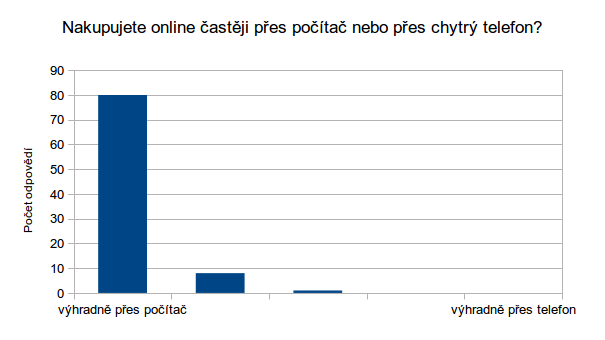
\includegraphics[width=400px]{img/pc-telefon}}\hypertarget{idp55147024}{}%
                                      \label{idp55147024}
                                  }
                                  {{\caption[{Rozložení odpovědí na otázku 
č. 20 -- počítač nebo telefon}]{{{Rozložení odpovědí na otázku č. 20 
-- počítač nebo telefon}}}\label{fig-smartphone}}}
                              \end{center}
                          \end{figure}

                          Zdánlivou drobností než skutečným podnětem 
k~inovaci je doporučení k~přezkumu všech textových označení 
v~zobrazovaných komponentách. Jak ukazuje obrázek 
\hyperlink{fig-sorting}{{\ref{fig-sorting}}}, původní popisek pro seřazení 
ceny \glqq vzestupně\textquotedblleft{} byl zvolen zcela nevhodně. O~něco 
málo srozumitelnější je z~pohledu uživatelů název \glqq nejnižší 
cena\textquotedblleft{}, nicméně zdaleka nejlépe zvolený popisek je \glqq 
od nejlevnějšího\textquotedblleft{}. Podobným způsobem je možné 
přezkoumat i další textové popisky, například již dříve zmíněný 
přechod do e-shopu označený jako \glqq Buy now\textquotedblleft{}.

                          % figure 
------------------------------------------------------
                          \begin{figure}[hbt]
                              \hypertarget{fig-sorting}{}%
                              \begin{center}

                                  
{{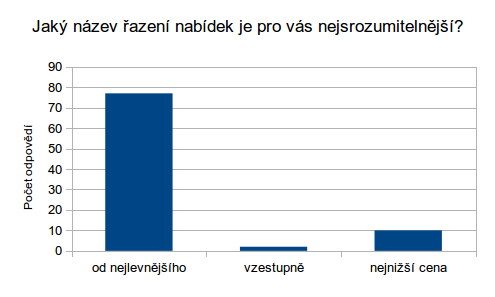
\includegraphics[width=380px]{img/sorting}}\hypertarget{idp55153968}{}%
                                      \label{idp55153968}
                                  }
                                  {{\caption[{Odpovědi na otázku č. 21 -- 
název řazení nabídek}]{{{Odpovědi na otázku č. 21 -- název řazení 
nabídek}}}\label{fig-sorting}}}
                              \end{center}
                          \end{figure}

                          Oblíbeným způsobem zobrazení affiliate odkazů 
v~rámci e-magazínů jsou i reklamní bannery a vyčleněné reklamní sloty 
na webové stránce. Odpovědi na otázku č. 23 ovšem ukazují, že 
efektivita takového odkazu a tedy následně sledovaný konverzní poměr jsou 
velmi nízké. Doporučujeme tedy primárně zobrazovat affiliate nabídky jako 
součást obsahu u~recenzí produktů, případně ve speciální sekci 
dedikované vyhledávání podle parametrů.
                          \subsection{Uživatelské komentáře}
                          \label{idp55156720}\hypertarget{idp55156720}{}%

                          Marketingový výzkum ukázal, že komentáře 
ostatních čtenářů jsou pro cílovou skupinu velmi důležitou součástí 
produktu. Nejčastější odpovědí respondentů je \glqq spíše 
ano\textquotedblleft{}, střední hodnota je dokonce vychýlena lehce k~\glqq 
určitě ano\textquotedblleft{}, jak ukazuje graf 
\hyperlink{fig-user-reviews}{{\ref{fig-user-reviews}}}. Žádný z~respondentů 
se nevyjádřil zcela negativně.

                          V~kapitole 
\hyperlink{sect-user-reviews-current}{{\ref{sect-user-reviews-current}}} byl 
popsán současný stav uživatelských komentářů. Je evidentní, že 
množství úsilí věnované této komponentě neodpovídá očekávání 
čtenářů. V~rámci inovace produktu je potřeba tuto část graficky vyladit 
a obohatit o~další funkcionalitu. Nejzákladnějším rozšířením je 
možnost reagovat na existující komentáře a tvořit tak diskusi. Čtenáři 
jinak používají pro reakce na konkrétní komentář značku zavináče 
s~uživatelským jménem autora, což sice k~rekonstrukci diskusního vlákna 
teoreticky vede, nicméně taková rozprava je absolutně nepřehledná.

                          Ačkoliv čtenáři nechtějí od e-magazínu, aby 
jim komentáře cenzuroval, určitá míra kontroly slušnosti a věcnosti je 
obecně očekávána, jak ukazují odpovědi na poslední otázku dotazníku 
s~číslem 25. Kromě samotného moderování diskuse administrátory a editory 
magazínu je možné zavést institut nahlašování nevhodných komentářů. 
U~každého příspěvku diskuse bude zobrazen vykřičník, vlajka nebo 
podobný symbol, kterým může kterýkoliv ze čtenářů upozornit na 
nevhodný komentář. Tímto se jednak zvýší podíl spoluvytváření 
produktu uživatelem (engagement), a zároveň tento přístup ušetří práci 
moderátorům. Užitečnou drobností pro správce diskuse může být také 
automatický systém, který automaticky nahlásí komentář obsahující 
některé z~předem specifikovaných výrazů -- vulgárních slov, ale i 
takových spojení, která často vedou k~nevhodné, například rasistické, 
diskusi.
                          \subsection{Rozšíření cílové skupiny}
                          \label{idp55164320}\hypertarget{idp55164320}{}%

                          Ačkoliv byla cílová skupina čtenářů TechRadaru 
společností Future identifikována jako muži, marketingový výzkum ukazuje, 
že ani ženy nelze z~potenciální cílové skupiny úplně vyloučit. Podle 
výsledků dotazníku sice ženy nakupují elektroniku na internetu pouze se 
zhruba třetinovou frekvencí než muži, a obdobně je snížena i částka, 
kterou takto utratí, nicméně pokud jde o~čtení recenzí a využívání 
cenových srovnání, není mezi oběma skupinami větší rozdíl. A~vzhledem 
k~tomu, že TechRadar není e-shop, ale e-magazín s~recenzemi, byla by chyba 
ženskou část opomenout.

                          Výsledky ukazují, že ženy mají tendenci 
prefereovat výběr z~širšího spektra. Sice nevyužijí například 
vyhledávání podle technických parametrů v~takové míře jako muži, ale 
pokud jde o~výběr na základě ceny nebo výše poštovného, mohou být 
ještě vhodnějším segmentem než muži. Právě výše poštovného je 
podle výsledků výzkumu jedním z~klíčových faktorů, podle kterého se 
ženy při nákupu elektroniky rozhodují. Pokud tedy e-magazín TechRadar chce 
rozšířit pole působnosti i na čtenářky, mohlo by být zajímavým 
řešením zahrnutí speciálních akcí, při kterých bude poštovné hradit 
e-shop. Takovéto akce e-shopy ve skutečnosti poměrně často pořádají, 
nicméně v~rámci e-magazínu a porovnáníní produktů jsou skryty mezi 
slevovými kupony, kterých je někdy až 70. Doporučením je tedy 
vyčlenění exkluzivních nabídek poštovného a označení takových 
produktů, resp. e-shopů.

  % -------------------------------------------------------------
  % Chapter Závěr 
  % ------------------------------------------------------------- MainMatter
\cleardoublepage
\phantomsection
\addcontentsline{toc}{chapter}{Závěr}
\chapter*{Závěr}
\markright{\contentsname}



                          V~rámci bakalářské práce byly shrnuty základní 
principy fungování affiliate marketingu. Následně byly popsány specifika 
nákupního chování a vývoje softwarového produktu, s~ohledem na specifika 
webového e-magazínu. V~praktické části byl zhodnocen současný stav 
provádění affiliate marketingu britskou vydavatelskou společností Future. 
Na základě prvotní analýzy byl sestaven marketingový výzkum mezi cílovou 
skupinou, na základě jehož výsledků byla formulována doporučení pro 
inovaci produktu.

                          Lze konstatovat, že základní očekávání 
cílové skupiny jsou současnou podobou produktu naplňována. Přesto byly 
identifikovány možnosti inovace produktu, zejména jeho rozšíření 
o~kvalitnější vyhledávání nabídek produktů. Část zabývající se 
prioritizací a řazením jednotlivých nabídek, reprezentovaných affiliate 
odkazy, ukazuje, že je možno současný řadící algoritmus rozšířit 
o~další vstupní parametry, jako je certifikát důvěryhodnosti e-shopu nebo 
zahrnutí i těch produktů, které nejsou momentálně dostupné, ale jejichž 
nabídka může být pro čtenáře i přesto zajímavá.

                          Formulovaná doporučení budou předána 
pracovníkům společnosti Future zodpovědným za provádění affiliate 
marketingu. Implementace některých inovací může být poměrně náročná 
(například personalizace týkající se reflektování pozitivních 
zkušeností s~konkrétním e-shopem), u~většiny vylepšení je ale 
technické řešení velmi snadné. Doporučení byla záměrně formulována 
tak, aby bylo možné je skutečně v~poměrně krátkém časovém horizontu 
vyvinout a nasadit v~nové verzi e-magazínu.

                          Pokud budou doporučení skutečně provedena, 
dalším logickým krokem je analýza výsledků těchto změn a jejich 
vyhodnocení. V~případě, že se inovace ukáže správnou, je zde možnost 
provedení další iterace vývoje produktu, tak jak bylo popsáno v~kapitole 
\hyperlink{sect-vyvoj-a-inovace}{{\ref{sect-vyvoj-a-inovace}}}. Inovaci 
produktu tohoto typu totiž nikdy nelze prohlásit za ukončenou. Stejně jako 
vydavatelé, kteří se včas neadaptovali na digitální prostředí, mají 
velké problémy, tak i ti, kteří nebudou elektronické verze svých 
magazínů pravidelně a znatelně inovovat, časem zjistí, že rychle se 
vyvíjející trh už je úplně jinde.

%									

%\cleardoublepage\chapter*{\uppercase{ZÁver}}
										
%								\phantomsection
%\addcontentsline{toc}{chapter}{\textbf{\uppercase{ZÁver}}}
%\markright{\contentsname}
										
	

\cleardoublepage
\renewcommand\bibname{Použitá literatura}

\bibliographystyle{unsrtnat}
\begin{thebibliography}{99}

\addcontentsline{toc}{chapter}{\textbf{\bibname}}
\markright{Použitá literatura}

% ............. biblioentry 
\bibitem{ab-testing}
KOHAVI, R. a LONGBOTHAM, R. a SOMMERFIELD, D. a HENNE, R.: \emph{Controlled experiments on the web: survey and practical
      guide}, Data Mining and Knowledge Discovery (Berlin: Springer)
        18 (1), 2009 [cit. 16. 3. 2014], Dostupné na {\textless}\url{http://ai.stanford.edu/~ronnyk/2009controlledExperimentsOnTheWebSurvey.pdf}{\textgreater}. 

% ............. biblioentry 
\bibitem{advertising-creative}
ALTSTIEL, T. a GROW, J.: \emph{Advertising creative: strategy, copy and design}, Los Angeles: Sage, 2010, 347 s., ISBN 9781412974912.

% ............. biblioentry 
\bibitem{am-impact}

DUFFY, D.: \emph{Affiliate marketing and its impact on e-commerce}, The Journal of Consumer Marketing, 22(2),
        s. 161-163, 2005 [cit. 9. 2. 2014], Dostupné po autentizaci na {\textless}\url{http://search.proquest.com/docview/220134240?accountid=16531}{\textgreater}. 

% ............. biblioentry 
\bibitem{amazon-cookie}

AMAZON: \emph{EU Associates Programme Operating Agreement}, 2013 [cit. 8. 2. 2014], Dostupné na {\textless}\url{https://affiliate-program.amazon.co.uk/gp/associates/agreement}{\textgreater}. 

% ............. biblioentry 
\bibitem{consumer-behavior}

SCHIFFMAN, L. a KANUK, L. a WISENBLIT, J.: \emph{Consumer behavior: global edition}, Boston: Pearson Prentice Hall, 2010, 592 s., ISBN 9780137006700. 

% ............. biblioentry 
\bibitem{copmlete-guide-to-am}

BROWN, B.: \emph{The Complete Guide to Affiliate Marketing on the Web}, Atlantic Publishing, 2009, 384 s., ISBN 978-1601381255. 

% ............. biblioentry 
\bibitem{customers-now}

SZETELA, D.: \emph{Customers Now}, iUniverse, 2009, 108 s., ISBN 978-1440170997. 

% ............. biblioentry 
\bibitem{dagmar}

COLLEY, R.: \emph{Defining Advertising Goals: For Measured Advertising
      Results}, The Association, 1961, 114 s., ISBN 978-0844234229. 

% ............. biblioentry 
\bibitem{decline-of-print}

KISSEL, M.: \emph{The decline of print doesn't mean the end of journalism}, 29. 10. 2013 [cit. 30. 3. 2014], The Guardian, Dostupné na {\textless}\url{http://www.theguardian.com/commentisfree/2013/oct/29/decline-print-media-journalism-web}{\textgreater}. 

% ............. biblioentry 
\bibitem{dh-test}

DOORNIK, J. a HANSEN, H.: \emph{An Omnibus test for univariate and multivariate normality}, Oxford Bulletin of Economics and Statistics,
        70, 2008, s. 927-939. 

% ............. biblioentry 
\bibitem{fcb-how-advertising-works}

VAUGHAN, R.: \emph{How Advertising Works: A~Planning Model}, Journal of Advertising Research, 20 (5), 1980, s. 27-33.. 

% ............. biblioentry 
\bibitem{fcb-how-advertising-works-slideshare}

BARCELO, J.: \emph{How Advertising Works}, SlideShare, 6. 3. 2010 [cit. 1. 3. 2014], Dostupné na {\textless}\url{http://www.slideshare.net/jcbarcelo/fcb-grid}{\textgreater}. 

% ............. biblioentry 
\bibitem{guardian-job-cut}

SWENEY, M.: \emph{Future Publishing to cut 55 jobs}, The Guardian, 3. 9. 2013 [cit. 8. 2. 2014], Dostupné na {\textless}\url{http://www.theguardian.com/media/2013/sep/03/future-publishing-cut-55-jobs}{\textgreater}. 

% ............. biblioentry 
\bibitem{independent-chris-anderson}

NICHOLAS, R.: \emph{Profile: Chris Anderson: Media with passion}, The Independent, 11. 7. 1999 [cit. 8. 2. 2014], Dostupné na {\textless}\url{http://www.independent.co.uk/news/business/profile-chris-anderson-media-with-passion-1105628.html}{\textgreater}. 

% ............. biblioentry 
\bibitem{internet-marketing-strategy}

CHAFFEY, D. a ELLIS-CHADWICK, F. a MAYER, R. a JOHNSTON, K.: \emph{Internet Marketing: Strategy, Implementation and Practice}, Pearson Education, 2009, 702 s., ISBN 9780273717409. 

% ............. biblioentry 
\bibitem{is-mu-redesign}

IS MU: \emph{Nový design zobrazení výsledků podobností}, Masarykova univerzita, 8. 10. 2013 [cit. 2. 3. 2014], Dostupné na {\textless}\url{https://is.muni.cz/blog/is_info/nov_20131008_podobnosti}{\textgreater}. 

% ............. biblioentry 
\bibitem{kotler-mm}

KOTLER, P.: \emph{Marketing Management}, Pearson Education, 2012, ISBN 978-0273755029. 

% ............. biblioentry 
\bibitem{lupa-datator}

SLÍŽEK, D.: \emph{Zkrocené Uloz.to má nástupce v~Datator.cz a historie se opakuje}, Lupa.cz, 7. 2. 2014 [cit. 8. 2. 2014], Dostupné na {\textless}\url{http://www.lupa.cz/clanky/zkrocene-uloz-to-ma-nastupce-v-datator-cz-a-historie-se-opakuje/}{\textgreater}. 

% ............. biblioentry 
\bibitem{managing-innovation}

TIDD, J. a BESSANT, J.: \emph{Managing innovation: integrating technological, market and
      organizational change}, Chichester: John Wiley \& Sons, 2009, 622 s., ISBN 978-0-470-99810-6. 

% ............. biblioentry 
\bibitem{marketing-performance}

FARRIS, P. a BENDLE, N. a PFEIFER, P. a REIBSTEIN, D.: \emph{Marketing Metrics: The Definitive Guide to Measuring Marketing
      Performance}, Upper Saddle River, New Jersey: Pearson Education,
        Inc, 2010, ISBN 978-0137058297.

% ............. biblioentry 
\bibitem{marketingova-komunikace}

FREY, P.: \emph{Marketingová komunikace: nové trendy 3.0}, Praha: Management Press, 2011, 203 s., ISBN 9788072612376. 

% ............. biblioentry 
\bibitem{navrh-vyzkumu}

PUNCH, K.: \emph{Úspěšný návrh výzkumu}, Praha: Portál, 2008, 230 s., ISBN 978-80-7367-468-7. 

% ............. biblioentry 
\bibitem{ols-asymptotic}

LUTZ, K. a DEMIROGLU, U.: \emph{Residual-Based Tests for Normality in Autoregressions: Asymptotic
      Theory and Simulation Evidence}, Journal of Business \& Economic Statistics 18
        (1), 2000, s. 40-50. 

% ............. biblioentry 
\bibitem{partnersky-program-seznam}

SEZNAM.CZ: \emph{Partnerský program Sklik}, 2014 [cit. 9. 2. 2014], Dostupné na {\textless}\url{http://napoveda.sklik.cz/cz/partner/}{\textgreater}. 

% ............. biblioentry 
\bibitem{performance-based-advertising}

DAINOW, B.: \emph{The rise of performance-based advertising}, iMedia Connection, 26. 3. 2008 [cit. 9. 2. 2014], Dostupné na {\textless}\url{http://www.imediaconnection.com/content/18800.asp}{\textgreater}. 

% ............. biblioentry 
\bibitem{personalisation}

REVERTE, C.: \emph{Personalization Innovators: Amazon, Netflix, and Yahoo!}, 28. 8. 2013 [cit. 26. 3. 2014], Dostupné na {\textless}\url{https://www.addthis.com/blog/2013/08/28/personalization-innovators-amazon-netflix-and-yahoo/}{\textgreater}. 

% ............. biblioentry 
\bibitem{razeni-inzeratu-seznam}

SEZNAM.CZ: \emph{Řazení inzerátů v~systému Sklik}, 2014 [cit. 9. 2. 2014], Dostupné na {\textless}\url{http://napoveda.sklik.cz/cz/zaciname-inzerovat/inzeraty-razeni/}{\textgreater}. 

% ............. biblioentry 
\bibitem{referral-marketing}

HRAJU, D.: \emph{Referral and Affiliate Marketing: What's the Difference?}, Referral Candy, 5. 11. 2010 [cit. 9. 2. 2014], Dostupné na {\textless}\url{http://blog.referralcandy.com/2010/11/05/referral-and-affiliate-marketing-whats-the-difference/}{\textgreater}. 

% ............. biblioentry 
\bibitem{rfc-cookie}

BARTH, A.: \emph{RFC 6265: HTTP State Management Mechanism}, University of California, Berkeley, 2011 [cit. 8. 2. 2014], Dostupné na {\textless}\url{http://tools.ietf.org/html/rfc6265}{\textgreater}. 

% ............. biblioentry 
\bibitem{spokojenost-lukasova}

LUKÁŠOVÁ, R.: \emph{Měření spokojenosti občanů s~veřejnými službami}, Masarykova univerzita, 2009 [cit. 9. 3. 2014], Dostupné na {\textless}\url{http://is.muni.cz/do/1456/soubory/oddeleni/svi/skripta/es2009-01.pdf}{\textgreater}. 

% ............. biblioentry 
\bibitem{theseus-paradox}

REA, M.: \emph{The Problem of Material Constitution}, The Philosophical Review, 104, 1995. 

% ............. biblioentry 
\bibitem{time-15-sec}
HAILE, T.: \emph{What You Think You Know About the Web Is Wrong}, 9. 3. 2014 [cit. 22. 3. 2014], Time Inc., Dostupné na {\textless}\url{http://time.com/12933/what-you-think-you-know-about-the-web-is-wrong/}{\textgreater}. 

% ............. biblioentry 
\bibitem{times-reuters}
POTTER, M. a HOLMES, D.: \emph{Paywall hits The Times online readership - paper}, Reuters, 18. 7. 2010 [cit. 9. 2. 2014], Dostupné na {\textless}\url{http://www.reuters.com/article/2010/07/18/newsinternational-times-idUSLDE66H09F20100718}{\textgreater}. 

% ............. biblioentry 
\bibitem{top-posting}
KASPRZAK, J.: \emph{Top Posting}, 9. 9. 2010 [cit. 15. 3. 2014], Dostupné na {\textless}\url{http://www.fi.muni.cz/~kas/blog/index.cgi/computers/top-posting.html}{\textgreater}. 

% ............. biblioentry 
\bibitem{twitter-redesign}
RUSSELL, J.: \emph{The redesigned Twitter.com has now rolled out to all users}, 
The Next Web, 4. 2. 2014 [cit. 2. 3. 2014], Dostupné na {\textless}\url{http://thenextweb.com/twitter/2014/02/04/the-redesigned-twitter-com-has-now-rolled-out-to-all-users/}{\textgreater}. 

% ............. biblioentry 
\bibitem{waterfall}

BENINGTON, H.: \emph{Production of Large Computer Programs}, IEEE Annals of the History of Computing 5
        (4), 1983 [cit. 9. 3. 2014], Dostupné na {\textless}\url{http://sunset.usc.edu/csse/TECHRPTS/1983/usccse83-501/usccse83-501.pdf}{\textgreater}. 

% ............. biblioentry 
\bibitem{youtube-mark-wood-interview}

FUTURE PLC: \emph{Mark Wood - November 2013 Interview}, YouTube, 16. 12. 2013 [cit. 8. 2. 2014], Dostupné na {\textless}\url{http://www.youtube.com/watch?v=W-EpxbH2KHY}{\textgreater}. 

% ............. biblioentry 
\bibitem{zvnonicek-monetizace}
ZVONÍČEK, P.: \emph{Monetizace webu}, Masarykova univerzita, 16. 3. 2013 [cit. 8. 2. 2014], Dostupné na {\textless}\url{http://www.fi.muni.cz/~xobsivac/PV219/prezentace11/monetizace.html}{\textgreater}. 


\bibitem{product-lifecycle-graph}
MR GOODACRE: \emph{PLC - The Product Life Cycle}, Mr Goodacre.com, 2013 [cit. 10. 3. 2014], Dostupné na {\textless}\url{http://www.mrgoodacre.com/plc---product-life-cycle.html}{\textgreater}. 


\end{thebibliography}


\newpage

\phantomsection

\renewcommand \listfigurename{Seznam grafů}
\renewcommand \listtablename{Seznam tabulek}
\newcommand{\listappendicesname}{Seznam příloh}
\newcommand{\appendices}[1]{\addcontentsline{apc}{appendices}{#1}}

\addcontentsline{toc}{chapter}{Seznam tabulek, grafů a příloh}
\markboth{Seznam tabulek, grafů a příloh}{Seznam tabulek, grafů a příloh}

\newlistof{appendices}{apc}{\listappendicesname}

\listoftables
\listoffigures
\listofappendices

%\phantomsection
%\addcontentsline{toc}{chapter}{Seznam tabulek}
%\markboth{Seznam tabulek}{Seznam tabulek}




%\chapter{Some Appendix}
%\appendix

\newpage
\chapter*{Přílohy}
\phantomsection
\addcontentsline{toc}{chapter}{Přílohy}
\markright{Přílohy}

\section*{Ukázky cenového srovnání v e-magazínu TechRadar}
\phantomsection

\hypertarget{appendix-screenshots}{}
\appendices{Ukázky cenového srovnání v e-magazínu TechRadar}

%\renewcommand{\figurename}{Ukázky cenového srovnání v e-magazínu TechRadar}
\begin{figure}[hbt]
    \hypertarget{fig-widget}{}%
    \begin{center}

        {{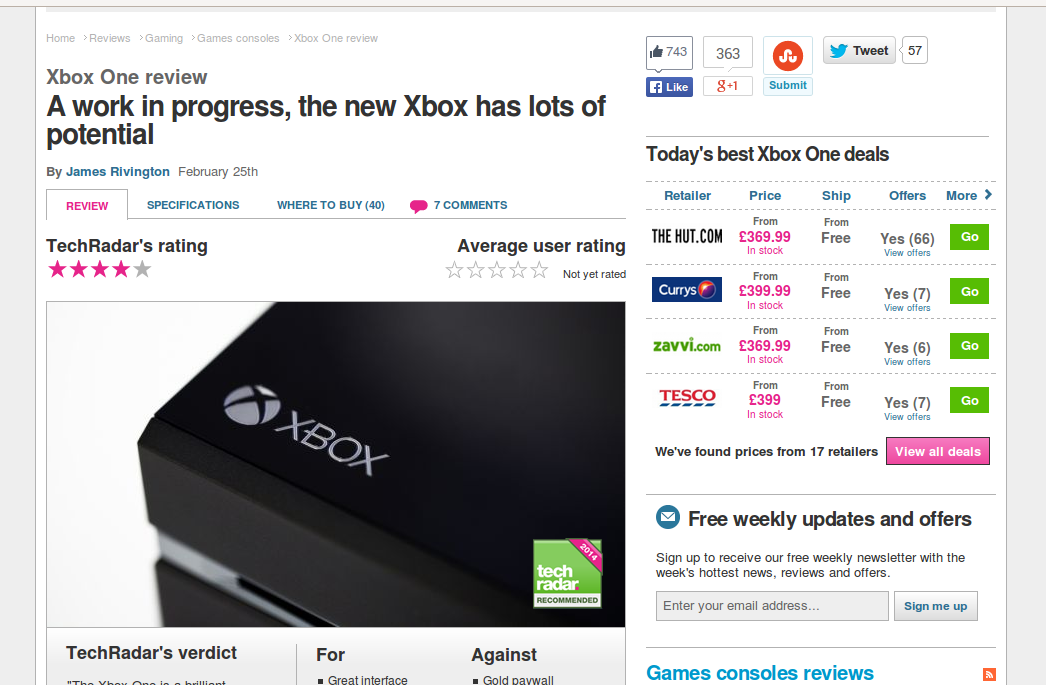
\includegraphics[width=450px]{img/widget}}\hypertarget{idp55374528}{}%
            \label{idp55374528}
        }
        {{\caption[{Cenové srovnání jako postranní komponenta přímo u~recenze}]{{{Cenové srovnání jako postranní komponenta přímo u~recenze}}}\label{fig-widget}}}
    \end{center}
\end{figure}

\newpage

% figure ------------------------------------------------------
\begin{figure}[hbt]
    \hypertarget{fig-price-comparison}{}%
    \begin{center}

        {{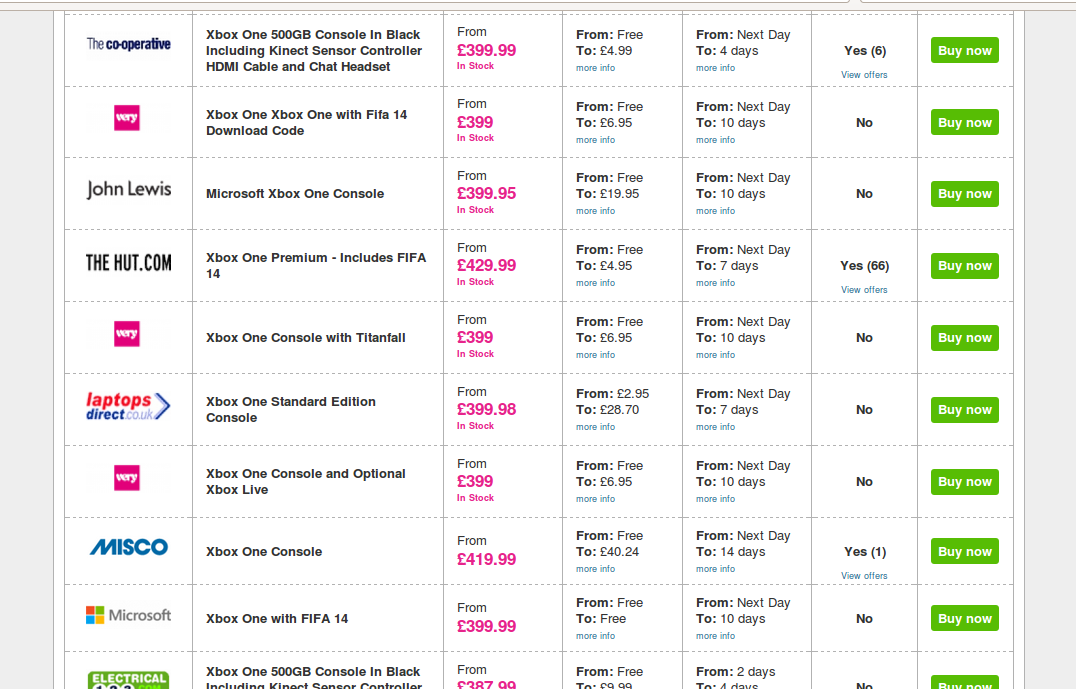
\includegraphics[width=450px]{img/price-comparison}}\hypertarget{idp55377360}{}%
            \label{idp55377360}
        }
        {{\caption[{Velká tabulka cenového srovnání}]{{{Velká tabulka cenového srovnání}}}\label{fig-price-comparison}}}
    \end{center}
\end{figure}


\newpage

\hypertarget{appendix-dotaznik}{}
\section*{Dotazník pro marketingový výzkum}
\phantomsection

\appendices{Dotazník pro marketingový výzkum}

Nakupování na internetu

Máte před sebou dotazník, který je součástí mé bakalářské práce. Dohromady má 25 otázek, jeho vyplnění by vám tak nemělo zabrat víc než 5 minut.

Pokud uvedete svou e-mailovou adresu, budete zařazeni do slosování a můžete vyhrát odměnu 500 Kč!

\begin{enumerate}

  \item Pohlaví
    \begin{itemize}
       \item Muž
       \item Žena
    \end{itemize}

  \item Kolikrát za rok nakupujete elektroniku (telefon, počítač, tiskárnu, foťák,~\ldots) online?
    \begin{itemize}
       \item Více než 5x
       \item 3x – 5x
       \item 2x
       \item 1x
       \item méně než 1x za rok
    \end{itemize}

  \item Kolik jste utratili za poslední rok za elektroniku na internetu? (částka v Kč)

  \item Kolik Vám je let?

  \item Jaké je Vaše nejvyšší dosažené vzdělání?
    \begin{itemize}
       \item Základní
       \item Středoškolské
       \item Vysokoškolské
    \end{itemize}

  \item Vaše e-mailová adresa (nepovinné, pouze pro účely slosování). 
      Odpovědi budou vyhodnocovány anonymně. 
      E-mailová adresa bude použita jen pro účely slosování a zaslání případné výhry 500 Kč.

  \item Než si vyberete nový počítač nebo televizi, pročítáte si internetové recenze?
    \begin{itemize}
       \item vždy
       \item většinou
       \item občas
       \item zřídka
       \item nikdy
    \end{itemize}

  
  \item Než si vyberete nový počítač nebo televizi, pročítáte si internetové recenze?
    \begin{itemize}
       \item vždy
       \item většinou
       \item občas
       \item zřídka
       \item nikdy
    \end{itemize}

\item Používáte internetové stránky porovnávající různé nabídky (cen) určitého produktu? (Například heureka.cz) 
    \begin{itemize}
       \item vždy
       \item většinou
       \item občas
       \item zřídka
       \item nikdy
    \end{itemize}

\item Vyhledáváte elektroniku podle různých parametrů (například laptop podle velikosti displeje či výrobce)? 
    \begin{itemize}
       \item vždy
       \item většinou
       \item občas
       \item zřídka
       \item nikdy
    \end{itemize}

  \item Myslíte si, že cenové srovnání by mělo zahrnovat nejen jeden vybraný produkt, ale i jeho možné alternativy? 
      Například kromě 3 nabídek telefonu "iPhone 5" z různých obchodů i srovnání podobného telefonu značky Samsung nebo Nokia.
    \begin{itemize}
       \item určitě ano
       \item spíše ano
       \item nevím
       \item spíše ne
       \item určitě ne
    \end{itemize}

  \item Chcete vidět fotky produktu, který vás zajímá?
    \begin{itemize}
       \item určitě ano
       \item spíše ano
       \item nevím
       \item spíše ne
       \item určitě ne
    \end{itemize}

  \item Pokud vidíte exkluzivní nabídku elektroniky, například s velkou slevou, neváháte a kupujete.
    \begin{itemize}
       \item vždy
       \item většinou
       \item občas
       \item zřídka
       \item nikdy
    \end{itemize}

  \item Je pro vás při nákupu elektroniky důležitá nízká cena? 
    \begin{itemize}
       \item určitě ano
       \item spíše ano
       \item nevím
       \item spíše ne
       \item určitě ne
    \end{itemize}

  \item Stačí vám vidět 5 nejlepších nabídek produktu, které za vás někdo vybral?
      Alternativou je, že preferujete si sami vybírat z desítek až stovek nabídek.
    \begin{itemize}
       \item určitě ano
       \item spíše ano
       \item nevím
       \item spíše ne
       \item určitě ne
    \end{itemize}

\item Používáte při nákupu slevové kupony (vouchery) dostupné na internetu?
    Slevové kupony jsou většinou součástí speciálních akcí, e-shopy je rozesílají třeba v newsletterech. 
    \begin{itemize}
       \item vždy
       \item většinou
       \item občas
       \item zřídka
       \item nikdy
    \end{itemize}

  \item Je pro vás při nákupu elektroniky důležitá dodací lhůta?
      Tedy za jak dlouho po nákupu Vám nový počítač nebo televizi přivezou domů.
    \begin{itemize}
       \item určitě ano
       \item spíše ano
       \item nevím
       \item spíše ne
       \item určitě ne
    \end{itemize}

\item Je pro vás při nákupu elektroniky důležitá doručovací cena (poštovné)?
    \begin{itemize}
       \item určitě ano
       \item spíše ano
       \item nevím
       \item spíše ne
       \item určitě ne
    \end{itemize}

  \item Pokud máte dobré zkušenosti s určitým e-shopem, budete ho příště preferovat?
    \begin{itemize}
       \item určitě ano
       \item spíše ano
       \item nevím
       \item spíše ne
       \item určitě ne
    \end{itemize}

  \item Důvěřujete více e-shopům s oficiálním certifikátem spolehlivosti?
    \begin{itemize}
       \item určitě ano
       \item spíše ano
       \item nevím
       \item spíše ne
       \item určitě ne
    \end{itemize}

  \item Nakupujete online častěji přes počítač nebo přes chytrý telefon?
    \begin{itemize}
        \item Odpovědi na škále 1 (výhradně přes počítač) - 5 (výhradně přes telefon)
    \end{itemize}

  \item Jaký název řazení nabídek je pro vás nejsrozumitelnější? Tedy jakému z těchto názvů porozumíte bez delšího přemýšlení
    \begin{itemize}
       \item od nejlevnějšího
       \item vzestupně
       \item nejnižší cena
    \end{itemize}

  \item Pokud není produkt momentálně skladem, ale jde o výhodnou nabídku, počkáte pár dní, než bude znovu k dispozici?
    \begin{itemize}
       \item vždy
       \item většinou
       \item občas
       \item zřídka
       \item nikdy
    \end{itemize}

  \item Stává se, že Vás reklama na webu zaujme a na reklamní banner kliknete?
    \begin{itemize}
       \item velmi často
       \item často
       \item občas
       \item zřídka
       \item nikdy
    \end{itemize}

  \item Je pro vás důležité hodnocení dalších lidí, kteří už si produkt zakoupili?
    \begin{itemize}
       \item určitě ano
       \item spíše ano
       \item nevím
       \item spíše ne
       \item určitě ne
    \end{itemize}

  \item Myslíte si, že by komentáře ostatních uživatelů měly být moderované?
      Tedy pokud někdo napíše např. vulgární komentář nebo uráží ostatní, provozovatel webu by ho měl smazat.
    \begin{itemize}
        \item Odpovědi na škále 1 (striktní dohled) - 5 (naprostá svoboda slova)
    \end{itemize}

\end{enumerate}


\end{document}
